\documentclass{sig-alternate-10pt}

\usepackage{times}
\usepackage{xcolor}
\usepackage{boxedminipage}
\usepackage{xspace}
\usepackage{pifont}
\usepackage{fancyvrb}
\definecolor{MyDarkBlue}{rgb}{0,0.08,0.45}
\usepackage[pdftex]{hyperref}
\hypersetup{
    colorlinks,%
    citecolor=MyDarkBlue,%
    filecolor=MyDarkBlue,%
    linkcolor=MyDarkBlue,%
    urlcolor=MyDarkBlue
}
\usepackage{fixltx2e}
\usepackage{textgreek}
\usepackage[sort]{cite}

\makeatletter
\newcommand*{\rom}[1]{\expandafter\@slowromancap\romannumeral #1@}
\makeatother

%,xcolor,rotating,graphicx,graphics,url,epsfig,
%amsfonts,algpseudocode,xspace,amsmath,amssymb,fancyvrb,fixltx2e

% Ethan hacks:----------
%\setlength{\pdfpagewidth}{8.5truein}
%\setlength{\pdfpageheight}{11truein}

%%% format things for making pretty tables using booktabs package
%\usepackage{multirow}
%\usepackage{booktabs}
%\setlength{\heavyrulewidth}{0.10em}
%\setlength{\lightrulewidth}{0.05em}
%\setlength{\cmidrulewidth}{\lightrulewidth}
%\setlength{\cmidrulekern}{0em}%
%
%\let\oldthebibliography=\thebibliography
%\let\endoldthebibliography=\endthebibliography
%\renewenvironment{thebibliography}[1]{%
%\begin{oldthebibliography}{#1}%
%\setlength{\itemsep}{-.3ex}%
%}%
%{%
%\end{oldthebibliography}%
%}

%\textfloatsep 10pt plus 3pt minus 2pt   % Space between main text and floats

%\newcommand{\squishlist}{
%   \begin{list}{$\bullet$}
%    { \setlength{\itemsep}{0pt}      \setlength{\parsep}{3pt}
%      \setlength{\topsep}{3pt}       \setlength{\partopsep}{0pt}
%      \setlength{\leftmargin}{1.5em} \setlength{\labelwidth}{1em}
%      \setlength{\labelsep}{0.5em} } }
%
%\newcommand{\squishlisttwo}{
%   \begin{list}{$\bullet$}
%    { \setlength{\itemsep}{0pt}    \setlength{\parsep}{0pt}
%      \setlength{\topsep}{0pt}     \setlength{\partopsep}{0pt}
%      \setlength{\leftmargin}{2em} \setlength{\labelwidth}{1.5em}
%      \setlength{\labelsep}{0.5em} } }
%
%\newcommand{\squishend}{
%    \end{list}  }
%
%
%\def\compactify{\itemsep=2pt \topsep=3pt \partopsep=1pt \parsep=1pt \leftmargin=1.5em}
%\let\latexusecounter=\usecounter
%\newenvironment{CompactEnumerate}
%  {\def\usecounter{\compactify\latexusecounter}
%   \begin{enumerate}}
%   {\end{enumerate}\let\usecounter=\latexusecounter}
%\newenvironment{CompactItemize}
%   {\def\usecounter{\compactify\latexusecounter}
%   \begin{itemize}}
%   {\end{itemize}\let\usecounter=\latexusecounter}
%

% Macros:
\newcommand{\projectname}{{STS}}
\newcommand{\projectmeaning}{the SDN Troubleshooting Simulator}

% Used to be: simulation-based causal inference
\newcommand{\simulator}{distributed delta debugging}
\newcommand{\Simulator}{Distributed delta debugging}
\newcommand{\SIMULATOR}{Distributed Delta Debugging}
\newcommand{\tbd}[1]{{\bf [[TBD: {#1}]]}}
\newcommand{\ie}{{\it i.e.}}
\newcommand{\eg}{{\it e.g.}}
\newcommand{\cf}{{\it cf.}}
\newcommand{\etc}{{\it etc.}}
\newcommand{\viz}{{\it viz.}}
\newcommand{\apriori}{{\it a priori}}
\newcommand{\eat}[1]{}

% Notes:
\newcommand{\num}[1]{{\color{red}\bf {#1}}}

\newcommand{\teemu}[1]{{\color{ForestGreen}\bf TK: {#1}}}
\newcommand{\andi}[1]{{\color{blue}\bf AW: {#1}}}
\newcommand{\sam}[1]{{\color{orange}\bf SW: {#1}}}
\newcommand{\colin}[1]{{\color{red}\bf CS: {#1}}}
\newcommand{\scott}[1]{{\color{purple}\bf SS: {#1}}}

%\newcommand{\teemu}[1]{}
%\newcommand{\andi}[1]{}
%\newcommand{\sam}[1]{}
%\newcommand{\colin}[1]{}
%\newcommand{\scott}[1]{}

% Signed quotes:
\def\signed #1{{\leavevmode\unskip\nobreak\hfil\penalty50\hskip2em
  \hbox{}\nobreak\hfil(#1)%
    \parfillskip=0pt \finalhyphendemerits=0 \endgraf}}

\newsavebox\mybox
\newenvironment{aquote}[1]
  {\savebox\mybox{#1}\begin{quote}}
    {\signed{\usebox\mybox}\end{quote}}

% Delta-debugging symbols:
\newcommand{\PASS}{\text{\ding{52}}\xspace}
\newcommand{\FAIL}{\text{\ding{56}}\xspace}
\newcommand{\cpass}{{T_{\scriptscriptstyle \PASS}}}
\newcommand{\cfail}{{T_{\scriptscriptstyle \FAIL}}}
\newcommand{\dpass}{{T'_{\scriptscriptstyle \PASS}}}
\newcommand{\dfail}{{T'_{\scriptscriptstyle \FAIL}}}
\newcommand{\test}{\textit{replay}\xspace}
\newcommand{\ddmin}{\textit{ddmin}\xspace}

\sloppy
\begin{document}
    \date{}

\title{How Did We Get Into This Mess?}
\subtitle{Isolating Fault-inducing Inputs to SDN Control Software}
    \author{Paper \#2, 14 pages}
    \maketitle
   \thispagestyle{empty}

% Advice from http://www.sigcomm.org/for-authors/hints-tips-and-guides/author-guide
%
%  Make sure the relevance to networking is clear. For instance, in a paper
%  describing a wonderful new protocol verification language, it is very easy
%  to get wrapped up in details of language syntax. Remember that SIGCOMM is a
%  networking conference, not a language conference, and ensure that how the
%  language improves the state of networking is made very clear.

\abstract{{\it The predominant technique for troubleshooting bugs in software-defined networks,
log analysis, is tedious and error-prone. We argue that a more principled
approach should be built around identifying inconsistencies between lower-level
network configuration and higher-level policies dictated by control
applications. Towards this end we present
cross-layer correspondence checking, a mechanism to automatically detect and
isolate inconsistencies due to bugs in the SDN platform. In
eventually-consistent systems such as SDN however,
transient inconsistencies between policy and configuration are inevitable.
We therefore augment correspondence checking with \simulator{} to help troubleshooters
distinguish pernicious persistent from harmless ephemeral inconsistencies. We
show that these techniques combine to help troubleshooters ``see through the fog'' of
diagnostic information.
}}

\section{Introduction}
\label{sec:intro}
The SDN platform's $raison\text{ }d'\hat{e}tre$ is to 
hide complexity from control applications. Modern controllers perform
replication, resource arbitration, failure recovery, and network 
virtualization on the control application's behalf. 

Despite the abstractions provided by the SDN programming model,
software-defined networks are no less complex than traditional networks. The architectural goal of SDN is
simply to push complexity from the control application onto the underlying platform.

SDN control platforms are prone to bugs as a result of their complexity. Bugs in the
platform present an architectural tension: troubleshooting requires
access to precisely the same details hidden by the platform's abstractions.
When an application developer 
encounters erratic behavior in the network, they must trace their
policy specification through multiple layers of abstraction
preceding changes in the physical network: virtualization logic,
distribution logic, and network devices. The error's root cause
may manifest in any of these layers, not just the control application.

As it stands, the SDN platform provides meager support for troubleshooting.
The predominant troubleshooting method is log analysis: manually
specifying log statements at relevent points throughout the system,
collecting, gathering, and ordering distributed log files, and analyzing the
results {\it post-hoc} when a error is encountered in production. Besides its
apparent tediousness, this approach is lacking in several ways: logs events
are enormous in number, impossible to aggregate into a single serial
execution of the system, and often at the wrong level of granularity to be of
use. \colin{</ why it's hard>}

Recent work has contributed much-needed improvements to this state of affairs. 
NICE applies concolic execution and model checking to SDN control
applications, thereby automating testing and catching bugs before
they are deployed~\cite{nice}. Aneater~\cite{anteater} and HSA~\cite{hsa}
introduce mechanisms for checking static invariants in the dataplane.
Nevertheless, no troubleshooting mechanism exists yet for the SDN platform itself.

New operating system abstractions face an arduous path towards adoption
without sound troubleshooting mechanisms. Analogously, the success of the
SDN programming model depends heavily on the utility of its troubleshooting
paradigm. Our goal in this paper is to work towards a useful
troubleshooting mechanism for the SDN platform. \colin{</ why it's important>}

We observe that in eventually-consistent systems such as sofware-defined networks,
transient inconsistencies are an inevitable property of the system.
Consequently, the process of troubleshooting errors essentially boils down to
identifying relevant events amongst a clamor of inconsistencies and diagnostic
information.

We present two mechanisms designed to make it easier for operators and
developers to ``see through the noise'' of diagnostic information. The first,
cross-layer correspondence checking, leverages the structure of the SDN
architecture to enable a general and verifiable notion of platform
correctness. Correspondence checking allows troubleshooters to isolate the cause of 
an inconsistency to a particular layer without needing to define invariants or
instrument third-party code. Our second
mechanism, simulated replay analysis, allows troubleshooters 
to differentiating ephemeral from persisent inconsistencies by steering the
execution of the system forward and backward in time, filtering out extraneous
external events, and inducing uncommon events such as failures. \colin{</ what we did>}

The rest of this paper is organized as follows. In \S\ref{sec:overview},
we present an overview of the SDN stack and its failure modes.
In \S\ref{sec:approach} we present correspondence checking and simulated
replay analysis in detail. In \S\ref{sec:evaluation} we present
two use-cases of our techniques, as well as a preliminary evaluation
of their runtime. Finally, in \S\ref{sec:related_work} we discuss related work,
and in \S\ref{sec:conclusion} we conclude.


\section{Context}
\label{sec:overview}
We begin by sketching the architecture of the SDN control plane and
illustrating the correctness challenges encountered by operators and
implementers.

SDN networks are managed by software running on a set of network-attached
servers called `controllers'. It is the job of the controllers to configure
the network in a way that complies with the intentions of network
operators. Operators codify their intentions by configuring
behavioral specifications we refer to as `policies'. Policy constraints
include connectivity, access control,
resource allocations, traffic engineering objectives, and middlebox
processing.

For fault-tolerance, production SDN control software is typically
distributed across multiple servers. For scalability, the responsibility for
managing the network can be partitioned through sharding.
Onix~\cite{onix}, for example, partitions a
graph of the network state across either an eventually consistent
distributed hash table or a
transactional database.
%allowing control applications to make their own
%tradeoffs in choosing consistency models and degree of fault tolerance.

In this distributed setting, controllers must coordinate amongst themselves
when reacting to state changes in the network or
policy changes from above.
Coordination in SDN is not exempt from the well-known class of faults
inherent to all distributed systems, such as
inconsistent reads, race conditions over message arrivals, and
unintended consequences of failover logic.

Several production SDN controllers support network
virtualization~\cite{bigswitch,nicirahomepage,contextream}, a technology that
abstracts the details of the underlying physical network and presents a
simplified view of the network to be configured by applications.
In this model, multi-tenancy is implemented by providing each tenant with their
own abstract network view, which are multiplexed onto the same physical network.
A common pattern is to treat an entire network as a single logical switch for each
tenant. When a large network is
abstracted in this way, the mapping between
the logical switch and the physical topology is highly complex.

In conjunction, the challenges of maintaining virtualized and distributed
objects while ensuring that critical invariants such as isolation between
tenants hold at all times make
SDN control software highly bug-prone.

To cope with these difficulties, software developers strive to thoroughly test
their software in a controlled environment before deploying to
production environments. The most common form of testing is unit testing,
where developers manually codify test cases to verify that individual software
components behave correctly. Each developer only has time to test a limited
number of cases though, and the number of test cases to consider is
practically unbounded, especially in
distributed systems. For this reason both of the SDN controller vendors we are
in contact with~\cite{nicirahomepage,bigswitch} employ a team of QA
engineers to automatically fuzz test~\cite{Miller:1990:ESR:96267.96279} their controller software
on a testbed of switches and hosts.
When a bug is discovered in the QA testbed, it is first triaged
by a human, then logs are collected and sent to a developer for further troubleshooting.

Troubleshooting bugs found through QA testing is often an arduous task,
despite the fact that many bugs developers deal with in practice
are mundane. Fuzz tests frequently run for many hours before bugs are found, and involve
a large number of distributed nodes. Moreover, QA testing frameworks do little to mitigate
non-determinism (and often introduce non-determinism of their own that
differs from what would be seen in production or on developer's local
machines), making it difficult for developers to replicate bugs.
Lastly, unlike the diverse set of tools available for debugging
individual programs, there are very few widely deployed debugging tools for
distributed systems~\cite{tooling_gap}; for highly non-deterministic bugs, it is not
uncommon for developers to throw
up their hands and simply wait until the next time the bug is observed before
continuing with diagnosis. We seek to improve this troubleshooting process.

In the next section we give a formal definition of our approach to
troubleshooting. We then spend
the bulk of the paper describing how we realize this formalism.

% \subsection{Environment / Workflow}
\andi{maybe discuss in Section 2 what our expected environment / workflow is, so people know what
to expect. Do we position this as a developer tool? What's our input?}

%--------------------------------------------------------------------%
%               OLD HOTNETS TEXT
\eat{

% Peter: useful to state your assumptions:
%is correct: policies, logical layer specification, physical layer model
%is possibly buggy: logical -> physical layer

We begin by sketching the architecture of SDN networks and
describing the failure-modes and correctness challenges encountered by operators and
implementers of SDN control platforms.

SDN networks are managed by software running on a set of network-attached
servers called ``controllers''. Modern SDN platforms differ from
`first-generation' controllers such as NOX~\cite{nox} in two aspects: they
maintain a virtualized view on top of which control
logic resides, and they distribute state across
multiple control servers.

%Two common patterns of control are proactive and
%reactive. Proactive controllers pre-compute forwarding tables for the entire
%network, and only push down updates periodically to react to link failures,
%changes in traffic mix, \etc. In contrast, in \emph{reactive} SDNs, the
%controller updates the forwarding state in reaction to a \emph{dataplane event},
%e.g., a previously unmatched patched found on the wire.

%Production SDN deployments are commonly proactive, primarily due to the large
%scale of datacenter networks and the current capabilities of forwarding
%hardware. We focus on proactive controllers for the remainder of this paper,
%although our troubleshooting mechanisms are also applicable to reactive
%applications.

\subsection{Virtualization Challenges}

\colin{Reviewer OA: might be interpreted as tied to a specific SDN platform.}

\colin{Reviewer OD: does this architecture allow you to specify performance
policies?}

Modern SDN controllers consist of at least three distinct layers, as depicted in
Figure \ref{fig:basicarch}. The two lower layers are part of the SDN platform.
The lowest layer maintains a graph data-structure known as the \emph{physical view}
that has a one-to-one correspondence with the physical network.
Synchronization logic in this layer keeps its information up-to-date with the
physical network state. Above, the \emph{logical view} translates the
potentially complicated physical network to a simpler logical view, commonly a single
logical switch~\cite{Casado:2010:VNF:1921151.1921162}. If the control platform supports virtualization, a
virtualization layer handles multi-tenancy by providing each tenant with their
own logical view, which are multiplexed onto the same physical network.
Finally, at the top of the stack
the \emph{control application} specifies the desired
high-level behavior of the network by configuring the logical view. We term these behavioral specifications
``policies''. Policy constraints might include connectivity, access control,
addressing resource allocations, traffic engineering objectives, or middlebox
processing.

The logical view greatly simplifies the job of specifying policies. However, SDN
does not reduce the overall system complexity; it merely moves complexity out of
the control application and into the platform, which must transform these
high-level policy specifications into the appropriate configuration of each
physical device. When an entire datacenter network (up to 10,000 switches) is
abstracted into a single logical switch, the mapping between the logical switch
and the physical topology is highly complex.
%; for example, a simple configuration
%change such as ``the path from $A$ to $B$ should pass through $C$'' must be
%implemented as routing entries in a sequence of switches in the physical
%network.

\eat{
This mapping is further complicated in a multi-tenant environment
\cite{Casado:2010:VNF:1921151.1921162} where each tenant specifies policies on
their own logical switch. In such a case, each controller must deal with
multiple tenants, and each tenant's policies must be coordinated among multiple
controllers. Maintaining isolation between tenants is critical; updates to the
physical network must therefore be performed in a consistent fashion to ensure
that isolation breaches do not occur for any in-flight packets, despite hardware
failures and message delays.
}

\subsection{Distribution Challenges}

For fault-tolerance, production SDN control software is typically \emph{physically
distributed} on several control servers. For scalability, the responsibility for
managing the network can be partitioned through sharding between
several control servers. Onix~\cite{onix}, for example, partitions a
graph of the network state across either an eventually-consistent
distributed-hash table or a
transactional database, allowing control applications to make their own
tradeoffs in choosing consistency models and degree of fault tolerance.

Policy and state changes require coordination between controllers.
Coordination in SDN is not exempt from the well-known class of faults
inherent to all distributed systems, such as
inconsistent reads, race conditions over message arrivals, and
unintended consequences of failover logic.

In conjunction, the challenges of maintaining virtualized and distributed
objects while ensuring that critical invariants such as isolation between
tenants are upheld at all times makes the task of constructing
SDN control software highly complex and error-prone. We aim to provide a
technique to ease the process of troubleshooting bugs encountered in this
task.

\colin{Reviewer OE: Before we introduce so much new mechanism for
debugging networks, I'd like to see an analysis of the incidence of
these corner cases.}

\eat{
The large scale of these networks also means that
error events such as link failures or software crashes are common. Microsoft,
for example, reports 36M error events over one year across 8 datacenters, which
implies 8.5 error events per minute per
datacenter~\cite{Greenberg:2009:VSF:1592568.1592576}. 
}

\begin{figure}[t]
    %\hspace{-10pt}
    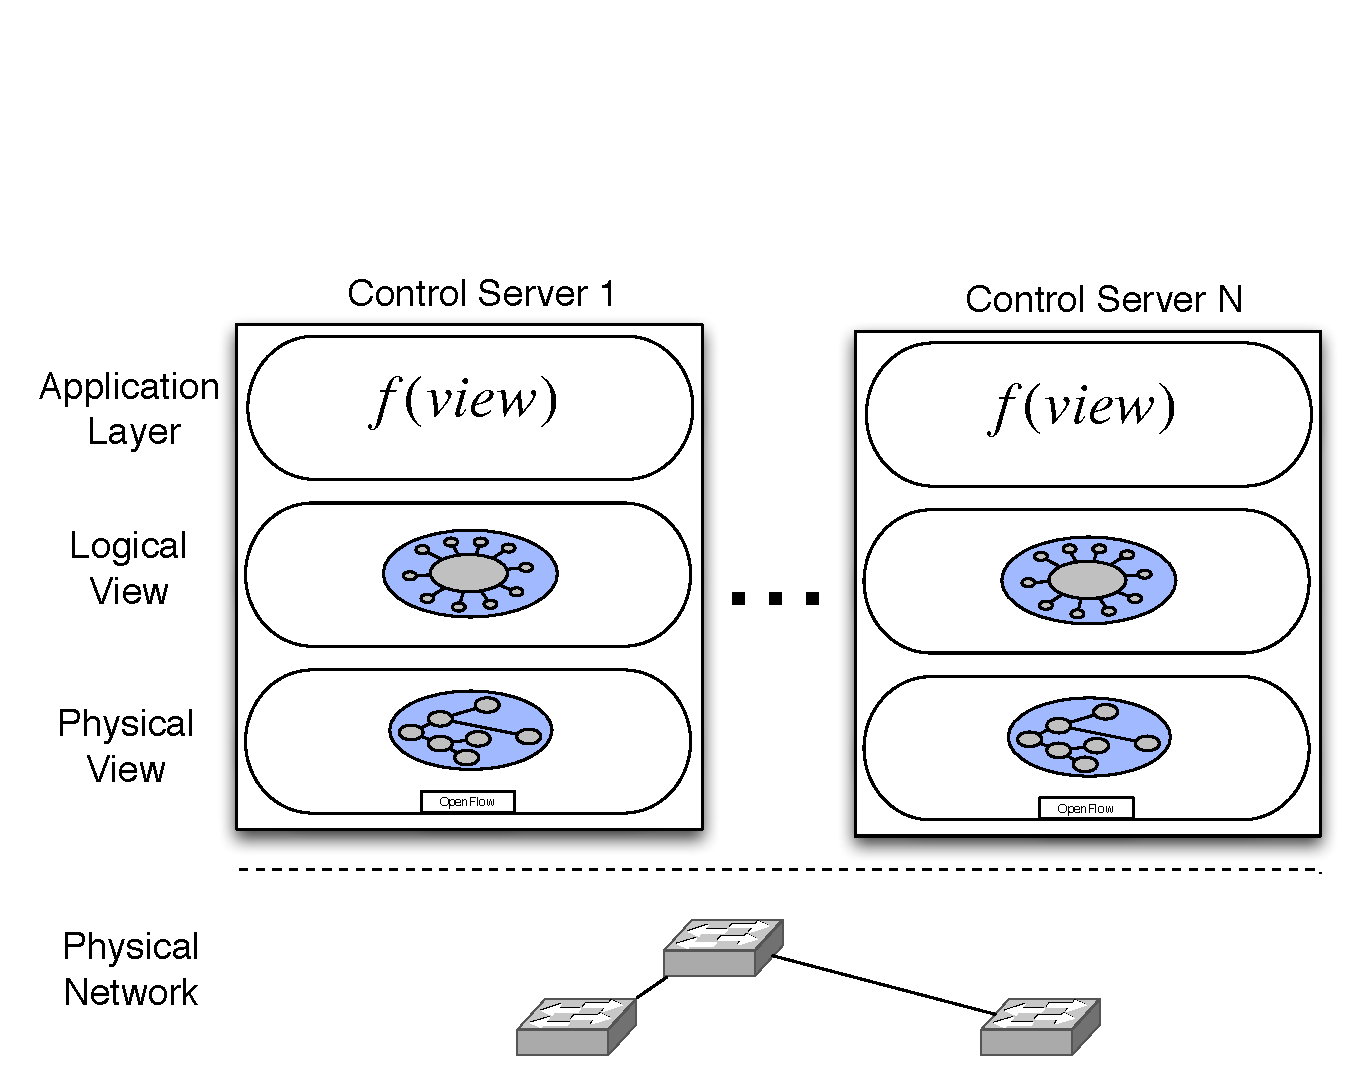
\includegraphics[width=3.25in]{../diagrams/architecture/SDN_Stack.pdf}
    \caption[]{\label{fig:basicarch} The SDN Software Architecture }
\end{figure}

\eat{
In this paper we focus on bugs in the virtualization and controller coordination
components of the SDN software stack. We focus on a \emph{proactive} mode of
operation where forwarding state updates are triggered by policy or topology
changes, not data-plane events.\footnote{It is possible to generalize our
approach to include inputs from the data-plane, subject to performance limitations.}
}

%We are primarily concerned with corner-case scenarios such as
%correlated hardware failures, which are the hardest to test {\it a priori}
%\andi{Check with our assumptions, i.e., uncorrelated external events}.
%Corner-case scenarios, while rare, cannot be ignored because of the distributed
%nature and large scale of production networks.
}


\section{Approach}
\label{sec:approach}
Given a log $(E_L, T_L, C_L)$ generated from testing infrastructure exhibiting an invariant violation,
our goal is to identify its MCS. This involves two tasks:
searching through subsequences of $E_L$, and searching for replay timings for those
subsequences that, if possible, trigger the original invariant violation.

\eat{
We introduce our approach using an example bug in the Floodlight open-source control
platform~\cite{floodlight_bug}. Floodlight is distributed across
multiple controllers for high availability, and provides support for
virtualization. Switches maintain one hot connection to a master controller and
several cold connections to replica controllers. The \emph{master} holds the
authority to modify the configuration of switches, while the other
controllers are in \emph{backup} mode and do not change the
switch configurations unless they detect that the master has crashed.

\begin{figure}[t]
  %\hspace{-10pt}
  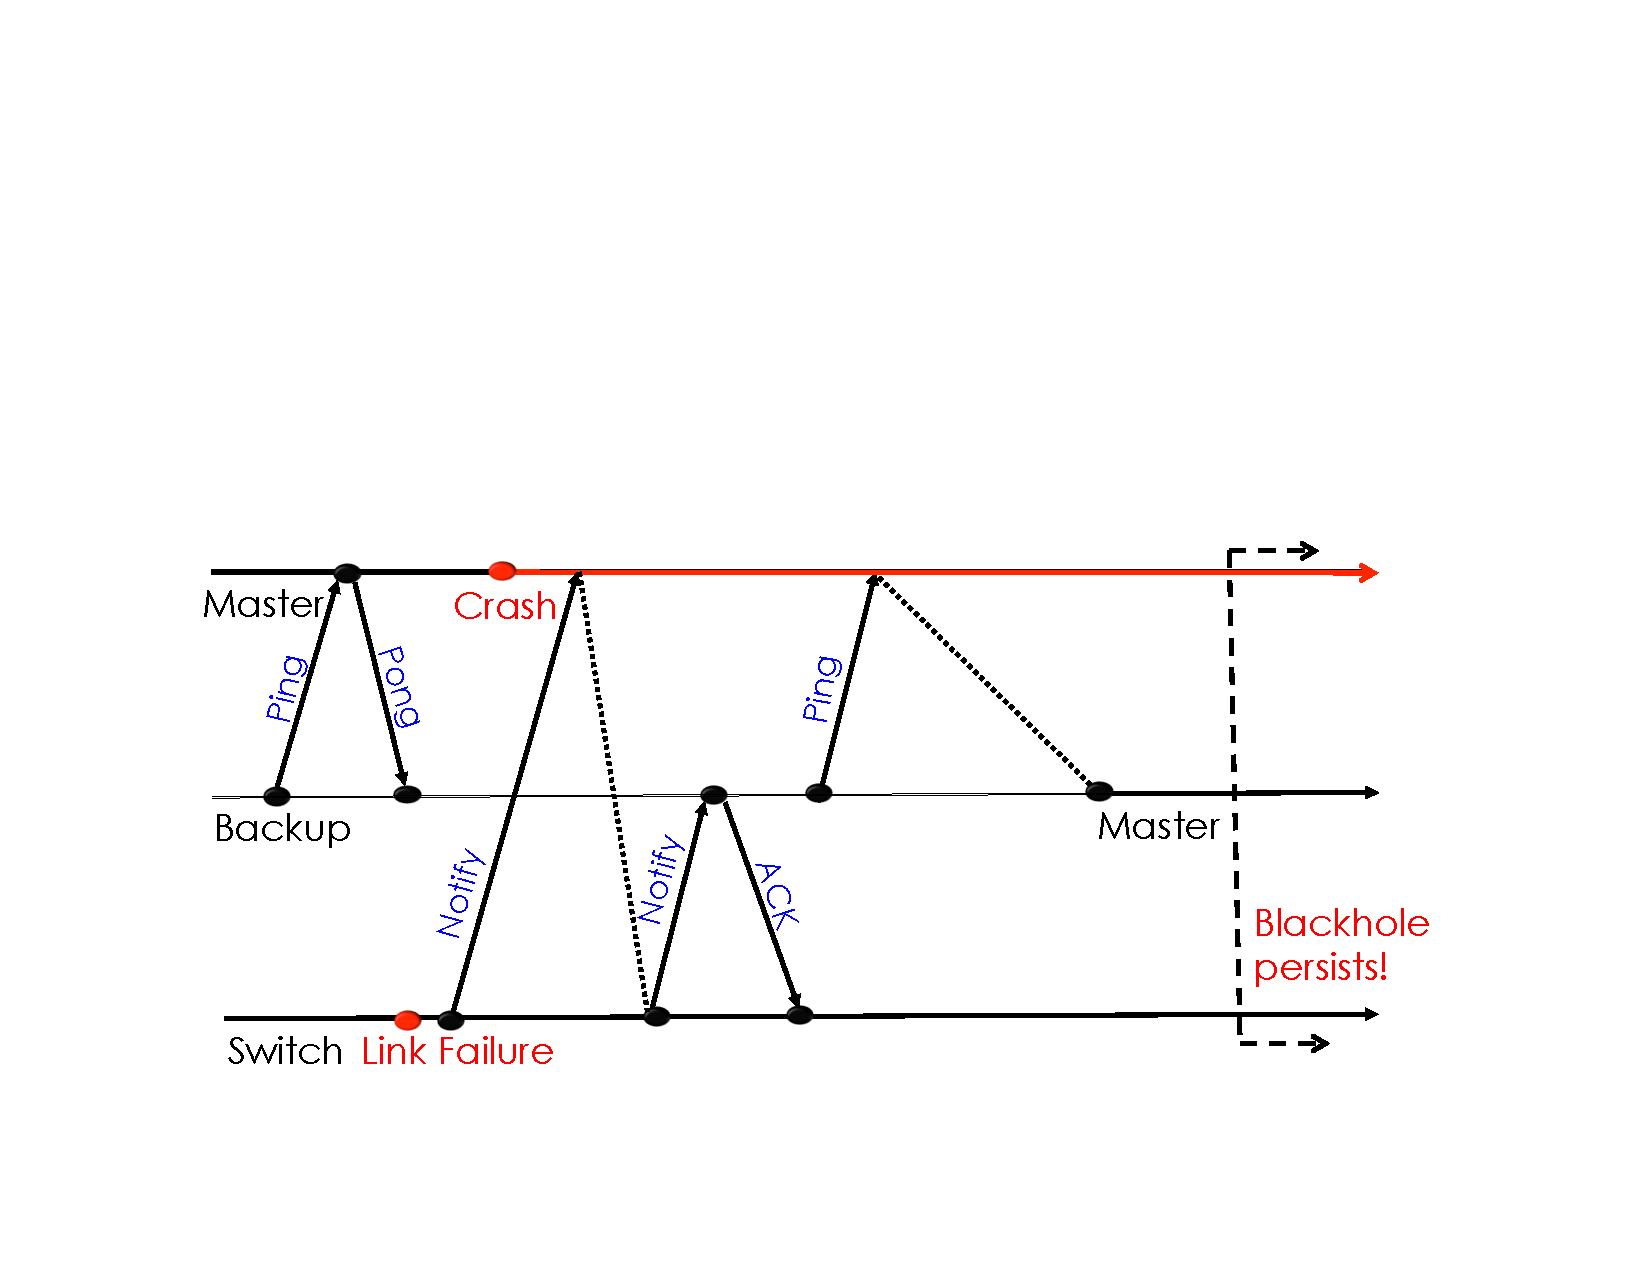
\includegraphics[width=3.25in]{../diagrams/case_study/example_bug.pdf}
  \caption[]{\label{fig:example} Floodlight failover bug. External inputs
             are depicted as red dots, internal events are depicted as black
             dots, and the dotted message line depicts a timeout.}
\end{figure}

The failover logic in Floodlight is incorrect, leading to the
following race condition\footnote{Note that this issue was
originally documented by the developers of Floodlight~\cite{floodlight_bug}.} depicted in
Figure~\ref{fig:example}:
a link fails (E1), and the switch attempts to notify the controllers (E2,E4) shortly after the master
controller has died (E3), but before a new master has been selected (E6). In this case, all live controllers are in
the backup role and will not take responsibility for updating the switch
flow table (E5). At some point, a backup notices the master failure and
elevates itself to the master role (E6). The new master will proceed to manage
the switch, but without ever clearing the routing entries for
the failed link, resulting in a persistent blackhole. In this example, the MCS
is the conjunction of the two external inputs (E1,E3).
}

\subsection{Searching for Subsequences}
\label{subsec:delta_debugging}

Checking random subsequences of $E_L$ would be one viable but inefficient
approach to achieving our first task. We do better by leveraging
%divide-and-conquer search technique from the software engineering community:
the delta debugging algorithm~\cite{Zeller:1999:YMP:318773.318946}, a
divide-and-conquer algorithm for
isolating fault-inducing inputs. In our case, we use delta
debugging to iteratively select subsequences of $E_L$ and replay each
subsequence with some timing $T$. If the bug persists for a given subsequence, delta debugging ignores the
other inputs, and proceeds with the search for an MCS within this subsequence.
%In what follows, we use the term {\em delta debugging} to refer to our algorithm for finding relevant subsequences.
The delta debugging algorithm is shown in Figure~\ref{fig:ddmin}.
%(with `$test$' replaced by `$replay$').

The input subsequences chosen by delta debugging are not always
valid. Of the possible inputs sequences we generate (shown in
Table~\ref{tab:inputs}), it is not sensible to replay a recovery event without a
preceding failure event, nor to replay a host migration
event without modifying its starting position when a preceding host
migration event has been pruned. Our implementation of delta debugging
therefore prunes failure/recovery event pairs as a single unit, and updates initial host locations
whenever host migration events are pruned so that hosts do not magically appear at new
locations.\footnote{Handling invalid inputs is crucial for
ensuring that the delta debugging algorithm finds a minimal causal
subsequence. The algorithm we employ~\cite{Zeller:1999:YMP:318773.318946}
makes three
assumptions about inputs: monotonicity, unambiguity, and consistency.
An event trace that violates monotonicity may contain events that ``undo'' the
invariant violation triggered by the MCS, and may therefore exhibit slightly
inflated MCSes. An event trace that violates unambiguity may exhibit multiple MCSes; delta debugging
will return one of them. The most important assumption is consistency, which
requires that the test outcome can always be determined.
We guarantee neither monotonicity nor unambiguity, but we guarantee consistency by
ensuring that subsequences are always semantically valid by applying the two
heuristics described above. Zeller wrote a follow-on
paper~\cite{Zeller:2002:SIF:506201.506206} that removes the need for these
assumptions, but incurs an additional factor of $n$ in complexity in doing so.}
These two heuristics account for validity of all network
events shown in Table~\ref{tab:inputs}. We do not yet
support network policy changes as events, which have more complex semantic
dependencies.\footnote{If codifying the semantic dependencies of
policy changes turns out to be difficult, one could just employ the more
expensive version of delta debugging to account for
inconsistency~\cite{Zeller:2002:SIF:506201.506206}.}

\begin{figure*}[t]
\begin{boxedminipage}{\textwidth}
Input: $\cfail$ s.t. $\cfail$ is a trace and $\test(\cfail) = \DFAIL$. Output: $\dfail
= \ddmin(\cfail)$ s.t. $\dfail \subseteq
\cfail$, $\test(\dfail) = \DFAIL$, and~$\dfail$ is minimal.
\begin{align*}
\ddmin(\cfail) &= \ddmin_2(\cfail, \emptyset) \quad \text{where} \\
\ddmin_2(\dfail, R) &=
\begin{cases}
\dfail & \text{\hphantom{else }if $|\dfail| = 1$ (``base case'')} \\
\ddmin_2\bigl(\done, R\bigr) &
\text{else if $\test(\done \cup R) = \DFAIL$ (``in $\done$'')} \\
\ddmin_2\bigl(\dtwo, R\bigr) &
\text{else if $\test(\dtwo \cup R) = \DFAIL$ (``in $\dtwo$'')} \\
\ddmin_2\bigl(\done, \dtwo \cup R\bigr) \cup \ddmin_2\bigl(\dtwo, \done \cup
R\bigr) & \text{otherwise (``interference'')}
\end{cases}
\end{align*}
\begin{center}
where $\test(T)$ denotes the state of the system after executing the trace $T$,
$\DFAIL$ denotes a correctness violation, \\
$\done \subset \dfail$, $\dtwo \subset \dfail$, $\done \cup \dtwo = \dfail$, $\done \cap
\dtwo = \emptyset$, and $|\done| \approx |\dtwo| \approx |\dfail| / 2$
hold.
\end{center}
\end{boxedminipage}
\caption{\colin{Cut if we need space} Automated Delta Debugging Algorithm From~\cite{Zeller:1999:YMP:318773.318946}}
\label{fig:ddmin}
\end{figure*}

\eat{ % Original O(n^2) algorithm
\begin{figure*}[t]
\caption{Minimizing Delta Debugging Algorithm From~\cite{Zeller:2002:SIF:506201.506206}}
\begin{boxedminipage}{\textwidth}
Input: $\cfail$ s.t. $\cfail$ is a trace and $\test(\cfail) = \FAIL$. Output: $\dfail
= \ddmin(\cfail)$ s.t. $\dfail \subseteq
\cfail$, $\test(\dfail) = \FAIL$, and~$\dfail$ is 1-minimal.
\begin{align*}
\ddmin(\cfail) &= \ddmin_2(\cfail, 2) \quad \text{where} \\
\ddmin_2(\dfail, n) &= 
\begin{cases}
\ddmin_2(\Delta_i, 2) & \text{\hphantom{else }if $\exists i \in \{1, \dots, n\} \cdot \test(\Delta_i) = \FAIL$ (``reduce to subset'')} \\
\ddmin_2\bigl(\nabla_i, \max(n - 1, 2)\bigr) & 
\text{else if $\exists i \in \{1, \dots, n\} \cdot \test(\nabla_i) = \FAIL$ (``reduce to complement'')} \\
\ddmin_2\bigl(\dfail, \min(|\dfail|, 2n)\bigr) & \text{else if $n < |\dfail|$ (``increase granularity'')} \\
\dfail & \text{otherwise (``done'').}
\end{cases}
\end{align*}
where $\test(T)$ denotes the state of the system after executing the trace $T$,
$\FAIL$ denotes a correctness violation, \\
$\nabla_i = \dfail - \Delta_i$, $\dfail = \Delta_1 \cup \Delta_2 \cup \dots \cup \Delta_n$, all
$\Delta_i$ are pairwise disjoint sequences of inputs, and $\forall \Delta_i \cdot |\Delta_i| \approx |\dfail| / n$
holds.
\end{boxedminipage}
\label{fig:ddmin}
\end{figure*}
}

\subsection{Searching for Timings}
\label{subsec:algorithm}

Simply exploring subsequences of $E_L$ is insufficient for finding MCSes: the
timing of those subsequences in each invocation of $replay()$ is crucial for reliably
reproducing the
invariant violation. The most natural approach would be to maintain the original
timings between the remaining original inputs for each subsequence.
\eat{\ie~if we
define $t_i$ as the timestamp of the $i^{th}$ input from the original run and $t'_i$ as the
replay clock value when it injects that same input
(which may or may not be the $i$'th input in the subsequence), then we might
just set $t'_i = t_i$.
\eat{
\begin{align*}
t'_0 = t_0 \\
t'_i = t'_{i-1} + |t_{i} - t_{i-1}|
\end{align*}
}
}
Unfortunately, this approach does not work in practice because it can violate
causal dependencies from the original execution, due to changes in the behavior
of the control software induced by pruning inputs. %\eat{: when we replay only a
%subsequence of the original inputs, the reaction of the control software
%can change, such that it behaves differently or takes a different amount of
%time to respond to the remaining inputs events.
%In practice we have observed that simply maintaining relative timings can
%result in injecting the remaining inputs too early or late.}
To reliably reproduce the invariant violation
we need to inject an input event $e$ only after all other
events, including internal events triggered by the control software itself,
that precede it in the
happens-before~\cite{Lamport:1978:TCO:359545.359563}
relation ($\{i \mid i \rightarrow e\}$) from the original execution have
occurred~\cite{tel2000introduction}.

Internal events include
(a) message delivery events, either between controllers (\eg~database
synchronization messages) or
between controllers and switches (\eg~OpenFlow commands), and (b) state transitions
within controllers (\eg~a backup node deciding to become master).
We obtain visibility into (a) by having our
\tester~(to be described in \S\ref{sec:systems_challenges}) interpose on all message channels.
We optionally obtain visibility into (b) by instrumenting controller
software with a simple interposition layer (to be described in \S\ref{subsec:mitigating}).
With visibility into internal events and control over input events, the
\tester~records a totally-ordered trace by logging an event only after
all prior events are completed.

%\subsection{Preserving Causality}

Maintaining the happens-before relation from the original trace
(which reproduces the violation) throughout replay of subsequences of the
trace (which may or may not reproduce that
violation) involves three issues: coping with syntactic differences in internal
events across runs,
handling internal events from the original
execution that may not occur after pruning, and dealing with new internal events that were not
observed at all in the original execution.

\eat{
\colin{Somewhat redundant. Maybe wait until use cases.}
While the inputs and original internal events are given to us,
we become aware of new internal events throughout replay by
(i) monitoring
control message receipts between controllers and switches,
and (ii) interposing on the controllers' logging library and notifying the
replayer whenever the control software executes a log statement (which serve to mark relevant state
transitions). Note that to achieve truly deterministic
replay, these log statements would need to
be highly granular, capturing information such as thread scheduling decisions;
we show in \S\ref{subsec:case_studies}
however that pre-existing, course granular log statements are often sufficient to
successfully reproduce bugs.}

%\footnote{We discuss this problem further in
%\S\ref{subsec:domain_knowledge}.}
%Note that the developer must provide enough logging statements
%so that relevant internal state transitions are captured and visible to our
%tool.

\begin{table}[tb]
\centering
\footnotesize
\begin{tabular}{|l|l|}
\hline
Internal message & Masked values \\
\hline
\hline
OpenFlow messages & xac id, cookie, buffer id, stats \\
% port numbers?
\hline
packet\_out/in payload & all values except src, dst, data \\
\hline
Log statements & varargs parameters to printf \\
\hline
\end{tabular}
\caption{Internal messages and their masked values. %The masks serve to
%define equivalence classes.
}
\label{tab:fingerprints}
\vspace{-0.5cm}
\end{table}


{\bf Functional Equivalence. } Internal events may differ syntactically (\eg~sequence numbers
of control packets may all differ) when replaying a subsequence of the original log.
We observe that many internal events are {\em functionally
equivalent}, in the sense that they
have the same effect on the state of the system with respect to triggering the
invariant violation (despite syntactic differences). For example, \emph{flow\_mod}
messages may cause switches to make the same change to their forwarding behavior
even if the transaction ids differ.

We leverage this observation by defining
masks over semantically extraneous fields of
internal events.\footnote{One consequence
of applying masks is that bugs involving masked fields are outside the purview of
our approach.} These masks only need to be specified once, and can later be
applied programmatically to event traces.

We show the fields we mask in Table~\ref{tab:fingerprints}. We consider an
internal event $i'$ observed in the replay
equivalent (in the sense of inheriting all of its happens-before relations) to an internal
event $i$ from the original log if and only if all unmasked fields have the same value
and $i$ occurs between $i'$'s preceding and succeeding inputs in the
happens-before relation.

\begin{table}[tb]
\centering
\footnotesize
\begin{tabular}{|l|l|}
\hline
\textbf{Input Type} & \textbf{Implementation} \\
\hline
\hline
Switch failure/recovery & TCP teardown \\
\hline
Controller failure/recovery & \verb=SIGKILL= \\
\hline
Link failure/recovery & \verb=ofp_port_status= \\
\hline
Controller partition & \verb=iptables= \\
\hline
Dataplane packet injection & Network namespaces \\
\hline
Dataplane packet drop & Dataplane interposition \\
\hline
Dataplane packet delay & Dataplane interposition \\
\hline
Host migration & \verb=ofp_port_status= \\
\hline
Control message delay & Controlplane interposition \\
\hline
Non-deterministic TCAMs & Modified switches \\
\hline
\end{tabular}
\caption{Input types currently supported by \projectname}
\label{tab:inputs}
\end{table}

\eat{
\begin{figure}[t]
    %\hspace{-10pt}
    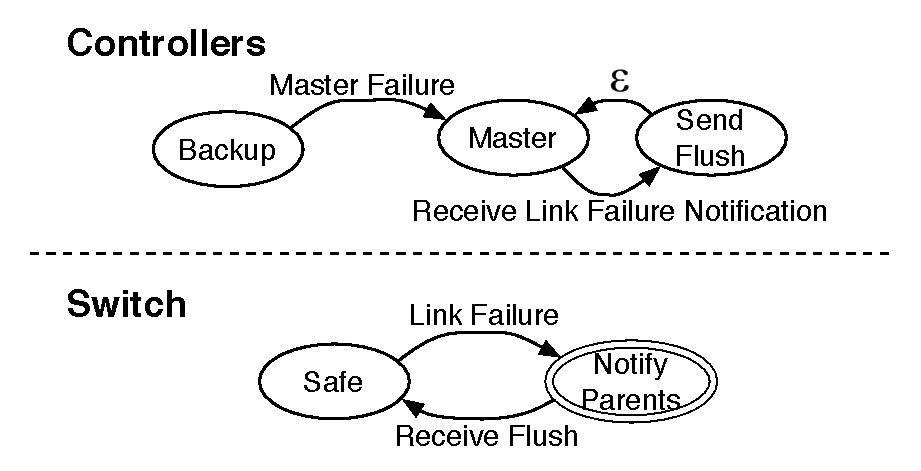
\includegraphics[width=3.25in]{../diagrams/state_machines/controller_switch.pdf}
    \caption[]{\label{fig:state_machines} Simplified state machines for the switch and
    controllers in the example Floodlight bug. Double outlined states
    represent presence of the blackhole.}
\end{figure}
}

{\bf Handling Absent Internal Events. } Some internal events from the original
log which causally ``happen before'' some external input
may be absent when replaying a subsequence of that log.
For instance, if we prune a link failure event, then
the corresponding link failure notification will never arise as an internal event.
\eat{
The control software's state machine (which we do not assume to know) determines whether
internal events cease to appear. Consider the simplified state machines for the switch and
controllers from the Floodlight case shown in
Figure~\ref{fig:state_machines}. If we prune the link failure input, the
master will never receive a link failure notification and
transition to and from \emph{Send Flush}.}

We handle this by attempting to infer the presence of internal
events before we replay each subsequence. Our algorithm (called {\sc Peek()}) for inferring the
presence of internal events is depicted in
Figure~\ref{fig:peek}. The algorithm injects each input, takes a
snapshot\footnote{We discuss the implementation details of snapshotting
in~\ref{subsec:snapshotting}.} of
the network and the control software's state, allows the system to proceed up
until the following input (plus a small time $\epsilon$), records the observed
events, and matches the
recorded events with the functionally equivalent internal events observed in
the original trace. With these inferred causal dependencies, we then replay
the subsequence, this time waiting to inject each input until each of its
(functionally equivalent) predecessors have occurred.\footnote{In the
case that, due
to non-determinism, an internal event occurs during {\sc Peek()} but does not occur
during replay, we time out on internal events after $\epsilon$ seconds of
their expected occurrence.}

\eat{ % Old version without peek()
We handle this possibility by waiting for each expected internal event
for a certain time \textepsilon. If the internal event does not occur within
this time, we assume that it is absent and proceed. If, however, we find
during the \textepsilon~time units we were waiting that another internal that
happens \emph{after} our next input occurs, we know that we have waited too
long and violated causality. In this case we need to restart the replay
process, this time knowing which internal events in the current
input interval are and are not going to occur before injecting the next input.
We show our overall event scheduling algorithm
in Figure~\ref{fig:replay}.
}

\eat{ % Somewhat redundant with peek()
\begin{figure}
  \begin{pseudocode}[framebox]{CausalInference}{events}
    \PROCEDURE{Replay}{subsequence}
    subsequence \GETS \CALL{Peek}{subsequence} \\
    \FOR e\textsubscript{i}\ in\ subsequence \\
      \BEGIN
      \IF e\textsubscript{i}\ is\ an\ internal\ event \\
      \AND e\textsubscript{i}\ is\ not\ marked\ absent:
      \THEN
        \BEGIN
          \Delta \GETS |e\textsubscript{i}.time - e\textsubscript{i-1}.time| + \epsilon \\
          wait\ up\ to\ \Delta\ seconds\ for\ e\textsubscript{i} \\
          \IF e\textsubscript{i}\ did\ not\ occur:
          \THEN mark\ e\textsubscript{i}\ as\ absent
        \END
      \ELSEIF e\textsubscript{i}\ is\ an\ input:
      \THEN
        \BEGIN
          \IF a\ successor\ of\ e\textsubscript{i}\ occurred: \\
          \INLINECOMMENT{waited too long}
          \THEN
            \RETURN{\CALL{Replay}{subsequence}}
          \ELSE
            inject\ e\textsubscript{i}
          \END
        \END
    \ENDPROCEDURE
  \end{pseudocode}
  \caption{{\tt Replay} is responsible for replaying subsequences of events
  chosen by delta debugging and determining
  if the bug reappears. \colin{Fix framebox width.}}
    \label{fig:replay}
\end{figure}
}

\begin{figure}
  \begin{pseudocode}[framebox]{Peek}{events}
    \footnotesize
    \PROCEDURE{Peek}{input\ subsequence}
    inferred \GETS [\ ] \\
    \FOR e\textsubscript{i}\ in\ subsequence \\
    \BEGIN
      snapshot\ system \\
      inject\ e\textsubscript{i} \\
      \Delta \GETS |e\textsubscript{i}.time - e\textsubscript{i-1}.time| + \epsilon \\
      record\ events\ for\ \Delta\ seconds \\
      matched \GETS original\ events\ \&\ recorded\ events \\
      inferred << e\textsubscript{i} << matched \\
      restore\ snapshot \\
    \END \\
    \RETURN{inferred}
    \ENDPROCEDURE
  \end{pseudocode}
  \caption{{\sc Peek} is responsible for determining which internal events
  from the original sequence are going to occur for a given subsequence.
  \label{fig:peek}}
\end{figure}

{\bf Handling New Internal Events.} The last possible change induced by pruning is the occurrence of new
internal events that were not observed in the original log.
New events present multiple possibilities for where
we should inject the next input. Consider the following case:
if $i_2$ and $i_3$ are internal events observed
during replay that are both in the same equivalence class as a single event $i_1$ from the
original run, we could inject the next input after $i_2$ or after $i_3$.

% TODO: figure this figure out
%\begin{wrapfigure}{c}{1.3\linewidth}
%  \centering
%  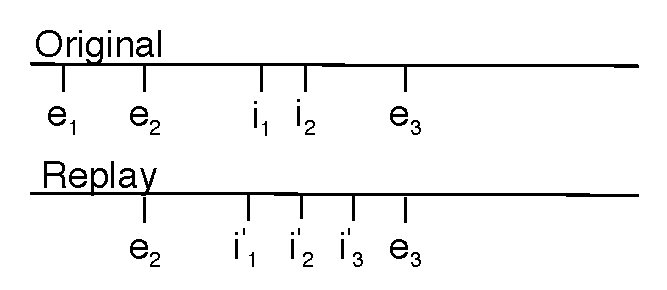
\includegraphics[width=\linewidth,height=0.8in]{../diagrams/state_machines/event_sequence.pdf}
%\end{wrapfigure}

In the general case it is always possible to construct two state machines that lead
to differing outcomes: one that only leads to the invariant violation when
we inject the next input
\emph{before} a new internal event, and another only when we inject \emph{after} a new internal
event. In other words, to be guaranteed to traverse any existing suffix that leads
to the invariant violation, we must recursively branch, trying both
possibilities for every new internal event. This implies an exponential number of
possibilities to be explored in the worst case.

Exponential search over these possibilities is not a practical option. Our heuristic when waiting for expected internal
events is to proceed normally if there are new internal events,
always injecting the next input when its last expected predecessor
either occurs or times out. This ensures that we always find suffixes that
contain a subset of the (equivalent) original internal events, but leaves open the
possibility of finding divergent suffixes that lead to the invariant
violation.
%This is reasonable because not even branching on new
%internal events is guaranteed to find the globally shortest fault-inducing input
%sequence:
%there may be other unknown
%paths through the state machine leading to the invariant violation that are
%completely disjoint from the original execution.

\eat{
Luckily, crucially ambiguous new internal events are not problematic for the
control software we evaluated, as we show in \S\ref{sec:casestudies}.
We conjecture that ambiguous new internal events are
rare because SDN software is a control plane system,
and is designed to quiesce quickly (\ie~take a small number of internal
transitions after any input event, and stop at highly connected vertices).
Concretely, SDN programs are often structured as (mostly independent) event
handlers, meaning that pruning input events simply triggers a subset of the original
event handlers.
\eat{
As an illustration, consider the state machines
in Figure~\ref{fig:state_machines}:
the controllers quickly converge to a single state (either ``Master'' or
``Backup''), as do the switches (``Safe'').
}
}

\subsection{Complexity}
\label{subsec:complexity}

The delta debugging algorithm terminates after $\Omega(\log n)$
invocations of $replay$ in the best case, and $O(n)$ in the worst case, where $n$ is the number of inputs in the original
trace~\cite{Zeller:1999:YMP:318773.318946}.
Each invocation of $replay$ takes $O(n)$ time
(one iteration for {\sc Peek()} and one iteration for the replay itself),
for an overall runtime of $\Omega(n \log n)$ best case and $O(n^2)$ worst case replayed inputs.
The runtime can be decreased by parallelizing delta debugging:
speculatively replaying subsequences in parallel, and joining the results.
Storing periodic checkpoints of the system state throughout testing can also reduce runtime, as it
allows us to replay starting from a recent checkpoint rather than the beginning of the
trace.% \barath{But doesn't this approach break due to non-determinism?  Sometimes we want
%a replay run to be different from a previous replay run...} 

\eat{
SDN platform developers can reduce the probability that the replay algorithm
will need to back up by placing causal annotations on internal
events~\cite{fonseca2007x}: with explicit causal information, the replay
algorithm can know
\apriori~whether certain internal events are dependent on pruned inputs.
}

\colin{Describe Andrew's input type pruning optimization and measurements. "We
make another optimization.."}

% In the next section we describe some of the practical challenges we have overcome to realize our approach.

% \colin{Cut this section?}
% In our initial experiments we have found that applying delta debugging to explore
% subsequences of $E_L$ and striving to maintain a single timing $T$ that maintains
% causal dependencies reliably finds small MCSes.


\section{System Design and Usage Scenarios}
\label{sec:architecture}
\projectname~(\projectmeaning) is our realization of the techniques described in
\S\ref{sec:approach}. \projectname~is implemented in roughly 10,000 lines of Python in
addition to the Hassel network invariant checking library~\cite{hsa}. The code
for \projectname~is publicly available.\footnote{URL omitted due to anonymity requirements}
Three industrial SDN companies to date have expressed interest in adopting it.\colin{Cite?}

In the rest of this section, we highlight salient points of \projectname's
design. Furthermore, we describe three ways \projectname~can be put to use
by SDN developers and operators.

The input types supported by \projectname~are shown in Table~\ref{tab:inputs}.
Controllers are notified of link, switch, and host migration events
via OpenFlow messages~\cite{openflow} sent by software switches.
Although the software switches do support packet forwarding, we
have chosen to de-emphasize dataplane performance in favor of
being able to simulate networks of large sizes. % as we show in \S\ref{subsec:runtime}.
% We hope to support policy changes in the future (Quantum)

\begin{table}
\centering
\begin{tabular}{|l|l|}
\hline
Link failure & Link recovery \\
\hline
Switch failure & Switch recovery \\
\hline
Control server failure & Control server recovery \\
\hline
Dataplane packet injection & Host migration \\
\hline
Control message delay & \\
\hline
\end{tabular}
\caption{Input types supported by \projectname}
\label{tab:inputs}
\end{table}

We designed \projectname~to be as resilient to non-determinism as possible
while minimizing modifications to control software.
\projectname ensures a deterministic order of messages despite
non-determinism in operating system I/O scheduling
by multiplexing all sockets in the controller process
onto a single true socket. \projectname~currently
overrides socket functionality within the control software itself, but
deterministic I/O could also be achieved without code modifications by
loading a shim layer on top of
libc (similar to liblog~\cite{Geels:2006:RDD:1267359.1267386}).

We also make a
small change to the control software's logging library\footnote{Currently
supported for POX
and Floodlight} to gain better visibility into the control software's internal state
transitions and achieve better replay synchronization: whenever a log
statement--a proxy for relevent state-changes--is executed, we
block the control software and notify \projectname~that a new state transition
is about to occur. \projectname then logs this event for later replay and
sends an acknowledgement to unblock the controller.
Additionally routing {\tt gettimeofday()} and {\tt getrand()} through
\projectname~makes replay more resilient to alterations in execution
speeds.\footnote{When the pruned trace differs from the original, we make a
best-effort guess at what the return values of these calls should be. For example,
if the altered execution invokes {\tt gettimeofday()} more times than were recorded
in the initial run, we interpolate the time values of neighboring events}
As an added benefit, overriding {\tt gettimeofday()} allows us to `compress'
runtime in some cases (similar to~\cite{Gupta06toinfinity}).

\projectname~can be used in a number of ways. We outline three use-cases here.

\subsection{Testing}

\projectname~is primarily used as a simulation and testing framework.
With complete control over event orderings, message drops, node
failures, \etc, \projectname~is especially useful for exploring corner cases
and ``what if'' questions. Along these lines, Amin Vahdat
has testified to the value of Google's SDN network simulator~\cite{vadhat}:
\begin{quote}
``One of the key benefits we have is a very nice emulation and
simulation environment where the exact same control software that would be
running on servers might be controlling a combination of real and emulated
switching devices. And then we can inject a number of failure scenarios under
controlled circumstances to really accelerate our test work.''
\end{quote}

In testing mode, \projectname~generates random or interactively chosen input
sequences, feeds them to controller(s), and monitors invariants at chosen
intervals. Driving the
execution of the system in this way allows \projectname~to record a
totally-ordered log of the events to be replayed later.

As additional failure cases are encountered they can be added
to a suite of integration tests and later used to validate the correct
behavior of future versions of the software. And because \projectname~makes
limited assumptions about the control software under test, the overall SDN community
could collect a repository of test cases to validate different SDN control platforms.

Automatically generating integration tests and identifying
minimal causal sequences frees developers to be more agile in
development, decreasing the time they spend writing test cases,
performing triage, and
hunting bugs. Beyond making test cases easier to reason about, minimal causal
sets serve to consolidate redundant test cases and thereby reduce time wasted
investigating bug reports the same root
cause~\cite{Zeller:2002:SIF:506201.506206}:
if two test failures have the same minimal causal sequence, it is
likely that the same underlying bug is being triggered.

\subsection{Replayable Traces}

When developers are unable to debug an issue, they often elicit help from
mailing lists or coworkers. The status quo today is to describe the conditions needed to
reproduce the bug as carefully as possible and hope that someone else is able
to replicate the issue.

With \projectname, developers can readily record errant executions and
exchange replayable traces with each-other.
Replayable traces shorten the debugging cycle, and increase chances that others
will be able to help. For example, bug reports can be filed with a replayable trace
attached, so that no
effort is wasted replicating the issue. With the help of print statements or a
debugger, developers can also iteratively run the trace as many times as
needed to identify the line(s) of code responsible for the problem.

\subsection{Forensic Analysis}

Perhaps the most valuable use case for \simulator~is forensic analysis of
production logs--correctness violations encountered in production are
high priority, and often time consuming to diagnose. While we have not
implemented this functionality, we present a sketch of
how forensic analysis could be performed with \simulator.

While \simulator~takes as input a single, totally-ordered log of the events in the
distributed system, production systems maintain a log at each node.
Instrumentation and preprocessing steps are therefore needed before \simulator~can be
invoked.

Production systems would need to include Lamport
clocks on each message~\cite{Lamport:1978:TCO:359545.359563} or have
sufficiently accurate clock
synchronization~\cite{corbett2012spanner} to obtain a partial global ordering
consistent with the happens-before relation.
Note that a total ordering is not needed, since it is permissible
for \simulator~to reorder concurrent events from
the production run so long as the happens-before relation is
maintained~\cite{Fischer:1985:IDC:3149.214121}.

The distributed logs would also need to make a clear distinction between internal events
(log messages, message sends/receipts), and input events (\eg~node failures). Further,
the input events would need to be logged in sufficient detail for \simulator~to
reproduce a synthetic version of the input that is indistinguishable to the control software
from the original input event. There will of course be some input events that cannot be reproduced
synthetically without significant complexity in what the simulator needs to model.
For example, suppose that the controller's faulty behavior is to flood a switch with messages,
causing the switch to drop some traffic. Yet only switches that are running low on memory
are affected by the controller's faulty behavior. To reproduce this failure mode correctly,
the simulator would need to model the memory levels of its software switches to match the
hardware behavior exactly.

Without care, a single input event may appear multiple times in the
distributed logs. A failure of the master node, for example, could be independently
detected and logged by all other replicas. The most robust way to
avoid redundant input events is to employ perfect failure
detectors~\cite{chandra1996unreliable}, which have the property that a
failure is logged iff
the failure actually occurred.\footnote{Perfect failure detectors are
typically implemented by explicitly killing slow
nodes.} Ensuring that a single failure detector is in charge of logging node failure
events guarantees that redundant inputs are eliminated. Alternatively, root cause analysis
algorithms~\cite{577079} or manual inspection could be employed to consolidate redundant
alarms.

Finally, some care may need to be taken to prevent the logs from growing so large that
\simulator's runtime becomes intractable. Here, causally consistent
snapshots~\cite{Chandy:1985:DSD:214451.214456} can minimize the number of inputs \simulator~needs
to examine. Specifically, with causally consistent snapshots of the distributed
system taken at regular intervals, \simulator~can bootstrap its simulation from the last snapshot before the failure.
If the MCS starting from this snapshot is empty, it can iteratively move backwards, starting from earlier
snapshots.\footnote{Technically the MCS may contain inputs from the very beginning of the execution. Arguably though,
the state that was induced by these inputs is reflected in each snapshot, and programmers would be able to detect
this by examining that state with a debugger.}

% --------------------------------------------------
%    OLD TEXT

\eat{

\subsubsection{Additional Use-Cases} Besides lifetime tracking and causal analysis, our simulation infrastructure has a
number of other possible use-cases:

\noindent\textbf{Checking related problems by fuzzing.} Input traces can be
\emph{fuzzed}~\cite{Miller:1990:ESR:96267.96279}, \ie{},
randomly perturbed, to expose the system to similar error conditions, and confirm
that a proposed solution is not just a point-fix. \colin{Need to be more clear
about what the constraints on the fuzzer are. (permutation or generation?)}

\noindent\textbf{Investigating pathological environment conditions.} The simulator allows for investigation
of pathological environment conditions difficult to achieve in a real world test bed
(\eg{}, correlated failure rates, extremely long delays etc.). This enables
investigation of situations that have a high potential for triggering errors.

\noindent\textbf{Interactive exploration.} Troubleshooters can also interactively bisect
the trace or modify specific events to further pinpoint the cause for a failure.
This is useful as soon as a suspect event sequence has been identified.

\noindent\textbf{Regression/Integration Test Library.} In traditional software engineering practices,
integration tests are an
important part of the software development cycle: developers feed end-to-end
input through the system, and verify that the system execution satisfies
certain safety and liveness properties. As additional failure cases are encountered in
production, new cases can be added to a suite of integration tests to
ensure robust operation of the system in future versions of the system.

Although the practice of accumulating an integration test suite over time is
commonplace in other fields of computer science, the field of networking
simply did not have the requisite software infrastructure to realize this practice before the emergence
of SDN. \Simulator{} can be viewed as our realization
of this development practice, applied to network controllers. Our simulator's fine-grained control over
failure scenarios allows us to test corner-case network conditions -- those
that are most difficult to anticipate in traditional unit tests.
As known failure cases are accrued over time, we envision \simulator{} being used to validate
new and existing SDN platforms.
}


\eat{

% Research question here?
% Going to be challenging to have this not come across as a software design
% spec.. Let's try to get this section over with as little text wasted as
% possible... I feel silly writing these sections, since I ALWAYS skip over
% them when I'm reading other people's papers...
\projectname{} is our realization of correspondence checking and \simulator{}
as a useful platform to troubleshoot SDN controllers. In this section we discuss
our goals in designing \simulator{}, and the challenges we encountered in the process
of realizing these goals.

\subsection{Design Goals: The 7 rules of \projectname{}}

We seek to build a system that facilitates the process of troubleshooting.
First and foremost, we hope that \projectname{} can reproduce difficult bugs
observed in production networks, and automate the process of diagnosing their
causes. We also envision \projectname{} being used as a common repository for difficult, corner-case
scenarios known to have caused problems for other control platforms in the
past. \colin{Redundant with "additional use-cases" section of approach}
Given these potential use cases, we require the design of the system to be
driven by the following requirements:

\noindent{\bf (1) Realistic Network Sizes.} We focus on large, production SDN
deployments. As today's datacenters may contain up to 100,000 hosts and 10,000
switches, our simulation infrastructure must be able to support large numbers
of switches.

\noindent \textbf{(2) Control plane focus} We expect the dynamism in our system to stem from
\emph{control plane events}. Typical rates of control plane events must thus be
handled, and control plane events must be modeled precisely. Conversely, we
don't expect to handle a realistic amount of dataplane traffic, which is
intractable for a software solution, and largely irrelevant in current networks
(because they are mostly proactive, so control planes are not being driven by packet arrivals).

\noindent \textbf{(3) Controller choice} Our system should run with existing production
controllers with minimum additional instrumentation. To allow for wider adoption, we don't want to limit ourselves to
a particular controller implementation.

\noindent \textbf{(4) Full determinism} We want our simulation environment to be fully
deterministic, such that repeated simulations with identical initialization values
yield provably identical results. This creates a challenge in conjunction with our goal (3).

\noindent{\bf (5) Comprehensive Failure Modes.} \projectname{} should
support a wide range of failure modes at all components in the
system, including switch and link failures and message drops, delays and reorderings.

\noindent\textbf{(6) Corner cases investigation} The potential state-space in a large-scale network
is intractably large \colin{Reviewer OD: do a better job of describing the
relationship of our work to model checking}.  We focus on interesting cases, as recorded, e.g., in production, or
found through interactive evaluation. To investigate related error conditions,
we \emph{fuzz} the input traces.

\noindent\textbf{(7) Interactivity} The system should be fast enough for interactive exploration through
an operator.

\medskip

While none of these requirements were particularly difficult in isolation, taken in aggregate they posed some difficulties, as we now recount.

\subsection{Components}

As depicted in Figure \ref{fig:system}, \projectname{} combines several
components to facilitate the process of troubleshooting SDN platforms:
\projectname{} takes input
from production traces, interactive manipulation, and synthetic trace
generation, and fuzzes these inputs to ensure that fixes are sufficiently general;
\projectname{}'s simulator supports large, sophisticated networks;
\projectname{} provides a deterministic, code-agnostic execution environment
for running SDN control software; and provides efficient algorithms for
checking correspondence throughout the system execution. We now provide an
overview of each of these components, and the challenges we encountered in
realizing our goals.

\begin{figure*}[!t]
  \centering
  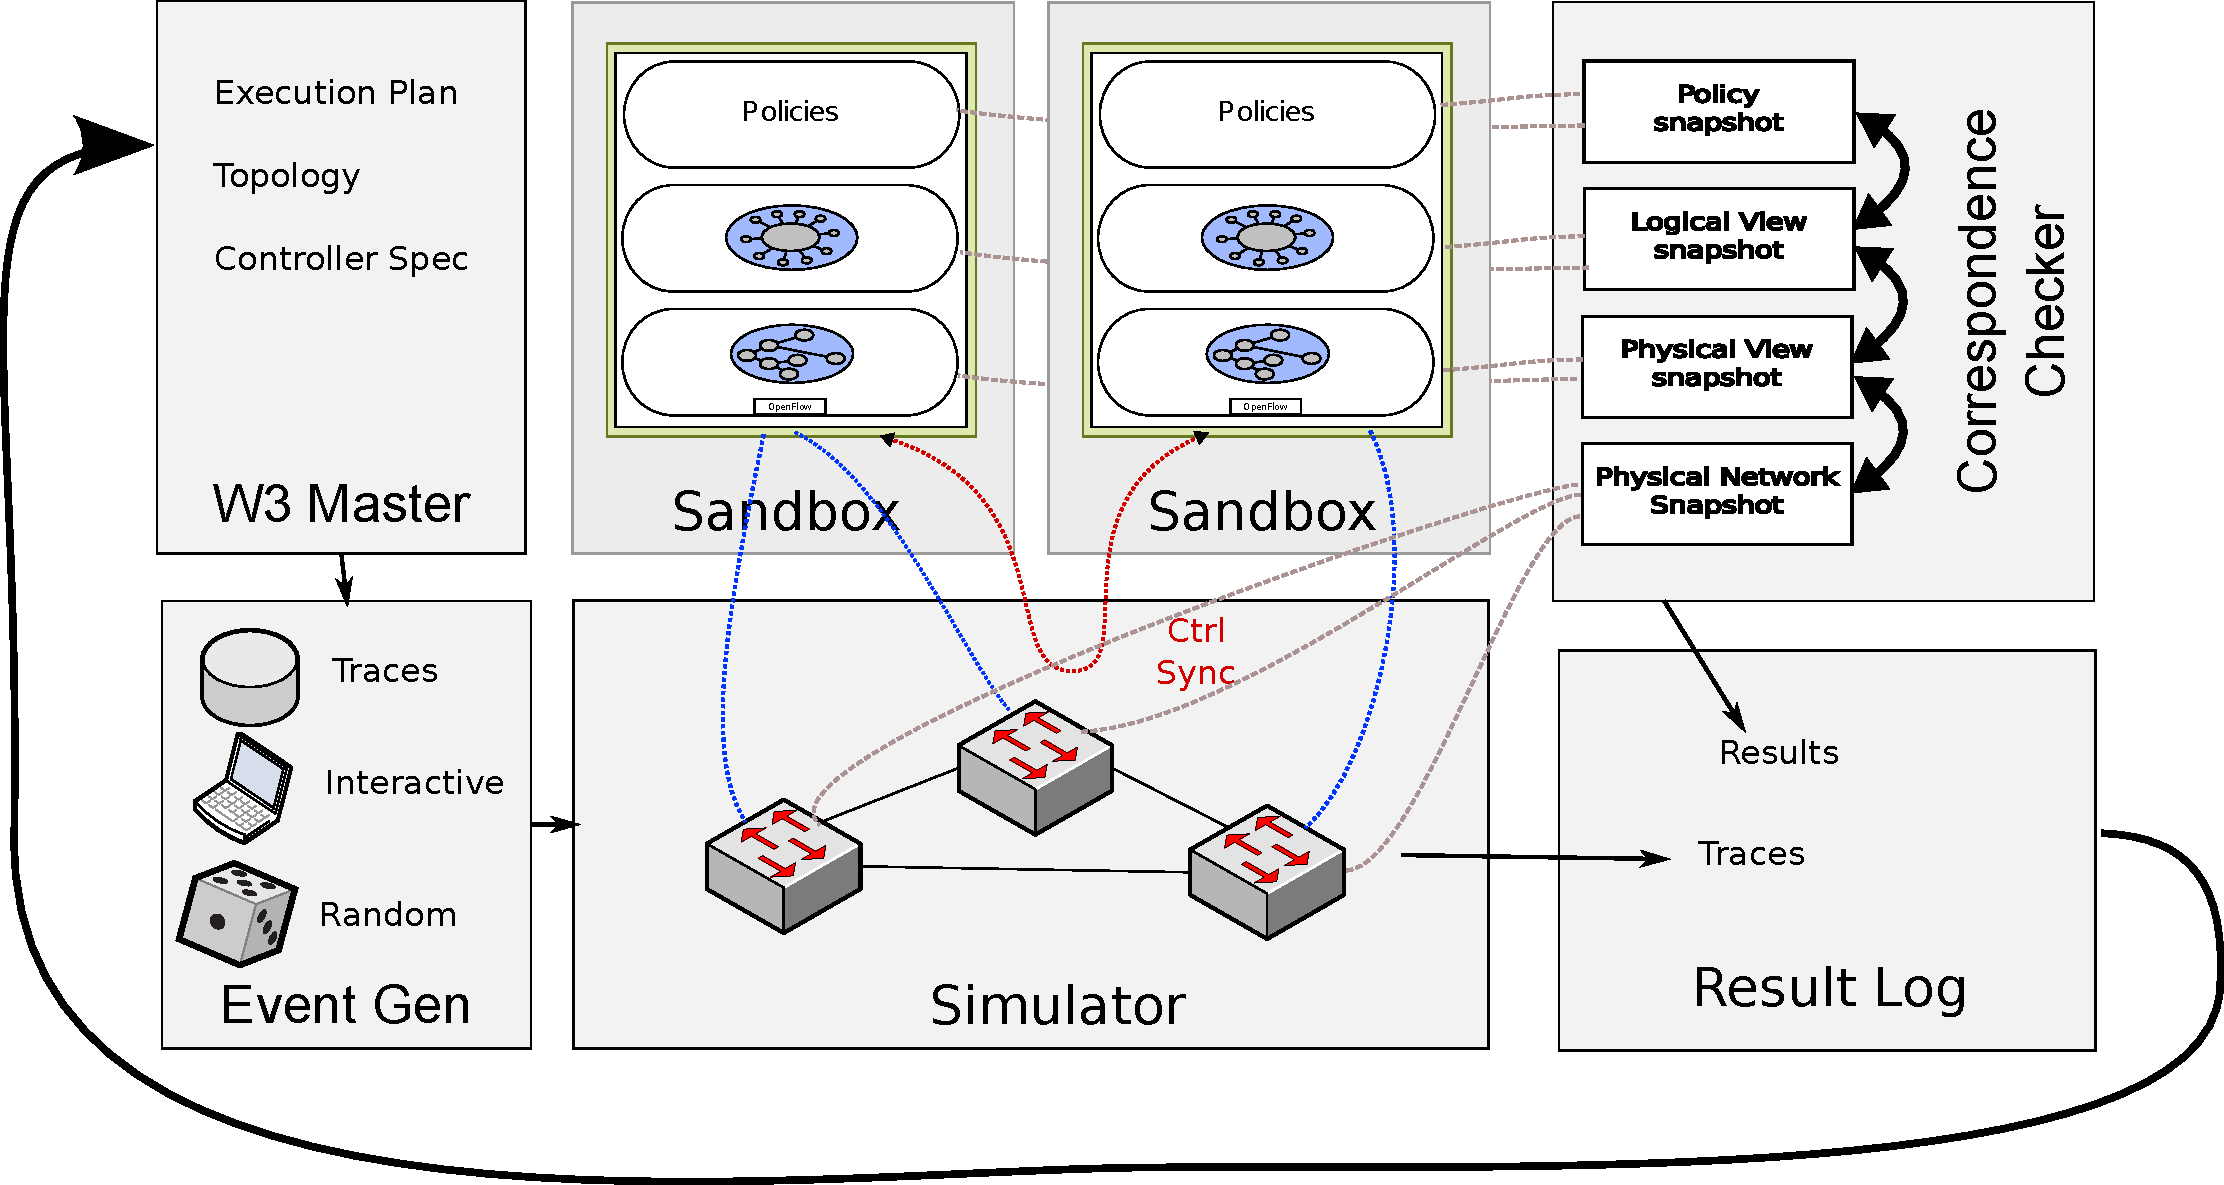
\includegraphics[width=0.8\textwidth{}]{../diagrams/architecture/architecture.pdf}
  \caption{System architecture. \colin{Andi: can haz new diagram? :P}}
  \label{fig:system}
\end{figure*}

\noindent{\bf Trace Input And Fuzzing.} Since a major goal of \projectname{} was
to support a wide range of usage scenarios, % WAT does that even mean
we provide support for three different methods for generating network trace
inputs. The most common method is to insert failure and topology change logs
from production deployments into the simulator for replay. Input traces may
also be produced synthetically with configurable, random probabilities for
network events. Lastly, we support interactive use, where the troubleshooter
has complete control over network events, and is thereby free to explore her
intuitions in order to reproduce a failure mode she has in mind.

\noindent{\bf Simulator.} We have built a simulator for SDN networks,
where network devices and hosts are modeled as lightweight python objects.
\colin{Reviewer OA: python objects creep in to the writing} Within a single thread, we
are able to deterministically model the execution of very large networks.
Our simulated model supports a wide
range of failure modes, and provides fine-grained control over event
orderings, component failures, and other aspects of the system execution. Our
simulator currently supports switch failures, link failures, arbitrary packet
re-orderings, drops and delays, and a fully general control plane.

The main challenge we encountered in the design of the simulator was
maintaining large numbers of TCP connections to the
controller(s). Although the controllers themselves may be spread
over multiple physical servers, the main simulator must nonetheless handle all
TCP connections between switches and controllers within a single process.
We ultimately ended up using epoll to avoid limitations of the UNIX select
implementation.

\noindent{\bf Controller Sandbox.} One of our major goals for \projectname{}
was to be able to run any SDN controller on top of the platform, with minimal
code changes to the controllers themselves. In addition, control servers
running on top of the simulated network must support deterministic execution
for reproducible results.

Currently we run applications as UNIX processes outside of the simulator.
We note however that there are a number of approaches for achieving deterministic
replay for external software. For example: a software determinism layer (e.g.
deterministic random number generators \colin{Reviewer OA: Whenever I see
replay, I worry about dealing with nondeterminism and pseudorandom number
generators. It was not clear how you are dealing with these issues.}) is
extremely lightweight, but requires modifications to the external software;
binary rewriting does not require any modification to the external
software's source code, but incurs moderate performance overhead; and VMs
fully support deterministic replay, but only a relatively small number of VMs can be run
on a single machine. We hope to leverage this previous work in future versions
of \projectname{}. Nonetheless, our architecture does not prevent us from
running controllers on different physical
servers in case we encounter memory or CPU bottlenecks.

\noindent{\bf Correspondence Checking.}
\projectname{} leverages the Hassel library provided by HSA~\cite{hsa}
to implement the correspondence checking algorithm. We optimize the code
slightly to run efficiently on large networks; in particular, we parallelize
symbolic packet propagation to a large number of subtasks. Correspondence
checking currently requires a small code change to the controller to fetch
the platform's view of the network state.

\projectname{} is written in roughly 10,000 lines of python, and is publicly
available. [anon]

}


\section{Evaluation}
\label{sec:evaluation}
\label{subsec:case_studies}

\begin{table*}
\centering
\begin{tabular}{l|l|l|l}
Bug Name & Topology & Replay Success Rate & MCS Size \\
\hline
Newly found Bugs & - & - & - \\
\hline
Pyretic loop & 3 switch mesh & TBD & 2 \\
% TBD
POX list removal & 2 switch mesh & 20/20 & 2 \\
% Total inpujts: 69
% With DP events: 72/2
% Original: config/eugene_epsilon_replay.py
% MCS: config/eugene_epsilon_mcs.py
POX in-flight blackhole & 2 switch mesh & 15/20 [20/20*] & 11 \\
% Total inputs: 26
% With DP events: 68/25
% Original: 7ba95ed82ca4e32f12ab511d9c4301dbac2c59d5
% MCS: 399cf861db87a65e600283d9ae7760400c4676e2
% Updated: updated_debug_branch_loop/
% TODO(cs): move to "known bugs"?
POX migration blackhole & 4 switch mesh & 20/20* & 3 \\
% Total inputs: 29
% With DP events: 117/3
% fuzz_pox_4mesh_blackhole
% Updated (fat tree): pox_fattree_migration
NOX discovery loop & 4 switch mesh & 18/20 & 18 \\
% Total inputs: 150
% With DP events: 358/58
% Original: ce547fc1df3bde279b6f3dd589c909663e295f1e
% MCS: 5f49e791b0c1a611454cf0930f54aa609dd635d3
% Updated to new format: nox_mesh_4_loop_repro_verbose
Floodlight loop & 3 switch mesh & 15/50 & 36 \\
% Total inputs: 284
% Andi
\hline
Known Bugs & - & - & - \\
\hline
Floodlight example failover bug & 2 switch mesh & N/A & 2 \\
% TBD: Ahmed
ONOS controller partition & TBD & TBD & TBD \\
ONOS forgotten flows & TBD & TBD & TBD \\
\hline
Synthetic Bugs & - & - & - \\
\hline
Load Balancer Flow Table Space & TBD & TBD & TBD \\
Ignored Bad OpenFlow args & TBD & TBD & TBD \\
Overlapping flow entries & TBD & TBD & TBD \\
Decision based on last byte of TCP SYN & TBD & TBD & TBD \\
Timer misfire & TBD & TBD & TBD \\
Algorithm misimplentation & TBD & TBD & TBD \\
Multithreaded race condition & TBD & TBD & TBD \\
Memory corruption & TBD & TBD & TBD \\
Failover bug & TBD & TBD & TBD \\
Consistency misunderstanding & TBD & TBD & TBD \\
Latency spike & TBD & TBD & TBD \\
Invalid sleep value & TBD & TBD & TBD \\
Non-deterministic TCAMs -> transient tenant isolation breach & TBD & TBD & TBD \\
\end{tabular}
\caption{Overview of Case Studies. \newline
\textmd{*with multiplexed sockets, overridden {\tt gettimeofday()}, and
logging interposition enabled.}}
\label{tab:case_studies}
\end{table*}

Our goal in this section is to show that \projectname~successfully produces
minimized event traces that are useful for troubleshooting. The
gold standard for evaluating \projectname~would be a large scale A/B test~\cite{neyman}
showing how much time it takes for developers to troubleshoot bugs found in
QA clusters with and without minimized event traces. Unfortunately
expert developers are scarce, and their skills vary widely; to achieve statistical significance we would
need hundreds of developers to spend substantial time on each bug we find.
%We also lack access to bugs found by QA testbeds of the scale and complexity
%used to test production controller software.

We instead take two approaches to evaluating \projectname.
First, we need to demonstrate \projectname's viability in
troubleshooting real bugs. We used \projectname~to find new bugs in \num{five} open source
SDN control platforms:
ONOS~\cite{ONOS} (Java), POX~\cite{pox} (Python), NOX~\cite{nox} (C++),
Pyretic~\cite{frenetic} (Python), and Floodlight~\cite{bigswitch} (Java), and
debugged these with \num{and without} the help of \projectname. Second, we demonstrate the
boundaries of where \projectname~works well and where it does not by using it to
troubleshoot synthetic bugs that span a range of bug types encountered in
practice. Throughout our evaluation we strive to qualitatively approximate A/B testing
with in-depth case studies on the troubleshooting process.

We show a high-level overview
of our results in Table~\ref{tab:case_studies}, and
illustrate in detail how \projectname~found their minimal causal sequences
in the rest of this section. Interactive visualizations and replayable event traces
for all of these case studies are publicly available (anonymized).

\subsection{New Bugs}

% \href{http://ucb-sts.github.com/experiments}{ucb-sts.github.com/experiments}.

\subsubsection{POX List Removal}
The first SDN control platform we examined was POX. %the successor of NOX. POX is
%a single-machine control platform intended primarily for research prototyping
%and educational use (\ie~not large scale production use). Nevertheless, POX has
%been deployed on real networks, and has a growing set of users.
The POX application we ran was a layer two routing module (`l2\_multi') that
learns host locations and installs exact match per-flow paths between known
hosts, after discovering links in the network. %, and a spanning tree module,
%which configures switches to only flood packets for unknown hosts along a
%spanning tree.

We start with a simple bug to illustrate that
\projectname~is useful for early stage development and testing.
We employed \projectname~to generate random sequences of
inputs, and found after some time that POX threw an exception due to
attempting to remove an element from a list where the element was not present.

There were $69$ randomly generated inputs in the trace leading up to the
exception. We invoked \projectname~to identify a two element MCS (runtime
shown in Figure~\ref{fig:list_runtime}):
a failure of a connected switch followed by a reboot/initialization of the same switch.
The stack trace made it easy to identify the code path that
immediately preceded the exception, and with
the knowledge that the initial triggering event was a switch failure we were able to
find why the original element was inserted into the list and fix the
problem within 15 minutes.

\begin{figure}[t]
    %\hspace{-10pt}
    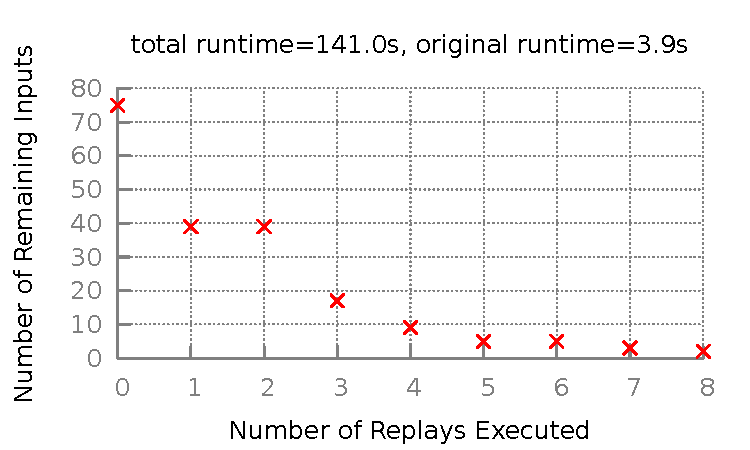
\includegraphics[width=3.25in]{../graphs/runtime/list_remove_error.pdf}
    \caption[]{\label{fig:list_runtime} Minimizing the POX list remove trace.}
\end{figure}

\eat{ % -----------------------------------
Apparently the developers of POX had not anticipated this particular event
sequence. Given the rarity of switch recovery events, and the tediousness of
writing unit tests for scenarios such as this
(which involved multiple OpenFlow initialization handshakes), this is not
surprising.
%Consider that the state-of-the-art open source technology for prototyping SDN
%applications, Mininet~\cite{handigol2012reproducible}, excels at
%testing common scenarios (on production OpenFlow software switches),
%but is not explicitly designed for scripting corner-case scenarios such as
%switch failure/recovery.
\projectname~made it straightforward to inject inputs
at a high semantic level,
and the minimized event
trace it produced made for a simple integration test.
} % -----------------------------------

%We illustrate type errors to show how STS is a useful framework for exploring
%code paths that you forget to unit tests.

\subsubsection{POX In-flight Blackhole}
We discovered the next bug after roughly 20 runs of randomly generated inputs.
We noticed that \projectname~reported a persistent blackhole while POX was bootstrapping its
discovery of link and host locations. There were $29$ inputs in the initial trace, and \projectname~returned a $11$ input
MCS (runtime shown in Figure~\ref{fig:pox_discovery}).

\begin{figure}[t]
    %\hspace{-10pt}
    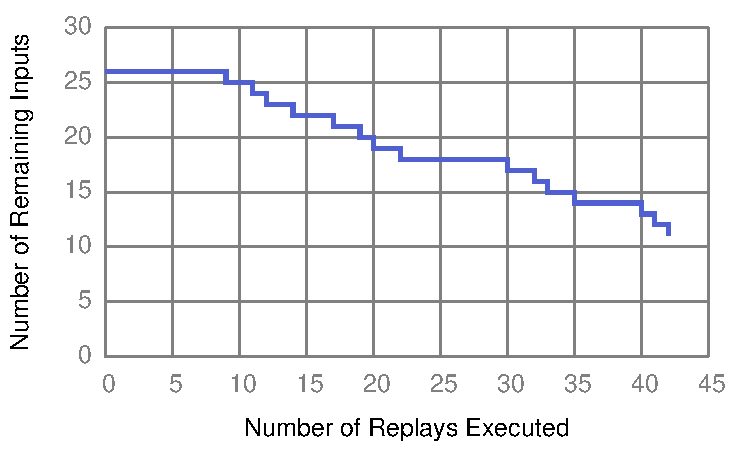
\includegraphics[width=3.25in]{../graphs/runtime/pox_blackhole.pdf}
    \caption[]{\label{fig:pox_discovery} Minimizing the POX in-flight blackhole.}
\end{figure}

We provided the MCS to the lead developer of POX. Primarily using the
console output, we were able to trace through the code and identify the problem
within 7 minutes, and were able to find a fix for the race condition within 40
minutes. By matching the console output with the code, he found that the crucial
triggering events were two
in-flight packets (set in motion by prior traffic injection events):
POX first incorrectly learned a host location as a result of the first in-flight
packet showing up immediately after POX discovered that port belonged to
a switch-switch link---apparently the code had not accounted for the
possibility of in-flight packets directly following link discovery---and
then as a result the
second in-flight packet
POX failed to return out of a nested conditional that would have
otherwise prevented the blackholed routing entries from being installed.

\eat{ % Maybe add this in -- it goes into much more depth. % -----------------------------------
We encountered this bug
on a simple topology, depicted in Figure~\ref{fig:simple_topo}, consisting of
two hosts A and B
and two switches S1 and S2 connected by a single link.

\begin{figure}[t]
    %\hspace{-10pt}
    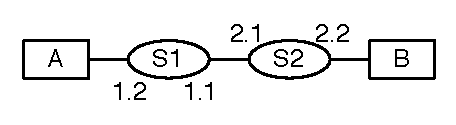
\includegraphics[width=3.25in]{../diagrams/state_machines/mesh_topo.pdf}
    \caption[]{\label{fig:simple_topo} Topology for POX
    in-flight blackhole. Numbers denote port labels.}
\end{figure}

Before the discovery module had learned of the link connecting the two
switches,
there were six traffic injection events between hosts (A$\rightarrow$ B and
B$\rightarrow$A). At the point when the link was discovered, POX had
previously learned
of B's location at port $2.2$, and correctly unlearned a previous location for
A at port $2.1$ (which it now knew to be a switch-switch link). %Upon POX would oscillate between learning the correct location
%of hosts at their ingress switch, and then learning an incorrect location
%when the flooded packet traversed the link and the next switch
%notified the controller of a new flow.\footnote{This seems to be necessary behavior before the
%links are discovered, since the hosts could have
%have legitimately migrated}
%This did not appear to be problematic though at first glance though,
%since we observed that POX correctly flushed the routing entries of the
%switches and forgot its incorrectly learned location of $A$ when it discovered
%that $1.1$ and $2.1$ were switch-switch ports, not host ports. At this point POX's only knowledge was the
%correct location of $B$ at $2.2$.

Directly after the link discovery we observed an {\em in-flight} packet arriving from A$\rightarrow$B at
port $2.1$
(without a prior flow notification from S1). This was POX's first error.
Upon examining the code, we found that it
did not account for in-flight packets concurrent with
link discovery. As a result,
POX incorrectly learned A's location at $2.1$, even though it knew that the link
could not have hosts attached. If the first packet had
instead originated at $1.1$, POX would not have made this mistake.

The next event we observed was another
{\em in-flight} packet from B$\rightarrow$A arriving at port
$1.1$. S1 notified POX of the unmatched flow, and POX appropriately printed a
log statement indicating that a packet had arrived at an internal switch port without a
previously installed flow entry. What happened next puzzled us though. POX
proceeded to install a path for this new B$\rightarrow$A flow, but the
path itself contained a loop: POX installed a B$\rightarrow$A entry going out both
$1.1\rightarrow2.1$ and $2.2\rightarrow2.1$, whereas it should have installed
only the latter (given A's current known location). The default behavior of
OpenFlow switches is to ignore matching route entries (with wildcarded in
ports) that forward out the
same port the packets arrived on. This is where we started observing the blackhole:
now whenever B sent traffic to A, it would be dropped at S1 until
the faulty routing entry would eventually expire $30$ seconds later.

We investigated the code that handled in-flight packets
arriving on switch-switch ports. The log statement that we had observed
earlier was inside a nested conditional, and the code for
installing the path was below and outside of the nested conditional.
What struck us was that there was a commented out return statement directly
after the log statement. The comment above it read: ``Should flood instead of
dropping''. We tried reinserting the return statement and replaying, and
the blackhole ceased to appear.

In summary, we found that the crucial triggering events were two
in-flight packets (set in motion by prior traffic injection events):
POX incorrectly learned a host location as a result of the first in-flight
packet, and
failed to return out of a nested conditional as a result the second in-flight
packet. We have sent the replayable trace generated by \projectname~to the lead
developer of POX, and await his response. We suspect that these fine-grained race conditions had not
been triggered before because message timing in
Mininet~\cite{handigol2012reproducible} or real hardware is not
delayed arbitrarily as it was in \projectname.

%We suspect this race condition was not observed in Mininet because the rate at which we were sending packets was
%significantly slower than in Mininet (which also sends $ARP$ and
%$IPV6$ pings), so that there were no in-flight flow notifications to POX to
%correct the situation.
% Discussion of how our gizmos helped.
} % \eat % -----------------------------------

\subsubsection{POX Migration Blackhole}
\colin{Move to "known bugs" section?}
Having examined the POX code in some depth, we noticed that there might be
some interesting corner cases related to host migrations.
We set up randomly generated inputs, included host
migrations this time, and checked for blackholes. Our initial input size was
$29$ inputs.
Before investigating the bug we
ran \projectname, and ended up with a $3$ input MCS (shown
in Figure~\ref{fig:pox_migration}): a packet injection from a
host (`A'), followed
by a packet injection by another host (`B') towards A, followed by a host migration of A. This made it immediately
clear what the problem was. After learning the location of A and installing a
flow from B to A, the routing entries in the path were never removed after A
migrated, causing all traffic from B to A to blackhole until the routing
entries expired.
%We did not know it at the time, but this was a known problem,
%and this particular routing module did not support host migrations. Nonetheless, this
%case demonstrates how the MCS alone can point to the root cause.

\begin{figure}[t]
    %\hspace{-10pt}
    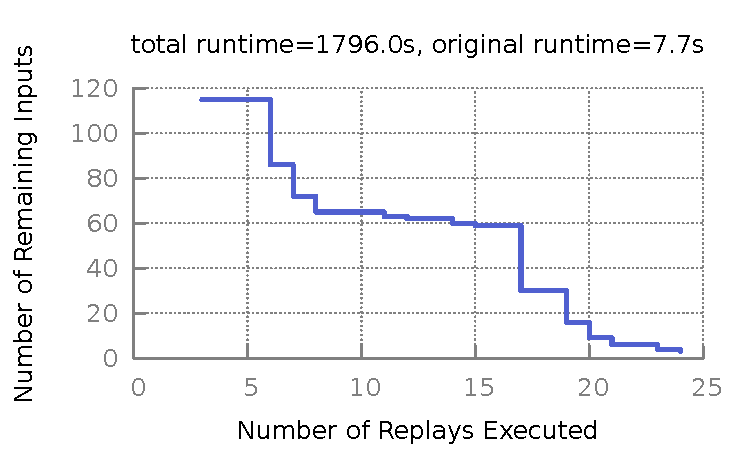
\includegraphics[width=3.25in]{../graphs/runtime/pox_migration_blackhole.pdf}
    \caption[]{\label{fig:pox_migration} Minimizing the POX migration
    blackhole.}
\end{figure}

\subsection{NOX Discovery Loop}

\begin{figure}[t]
    %\hspace{-10pt}
    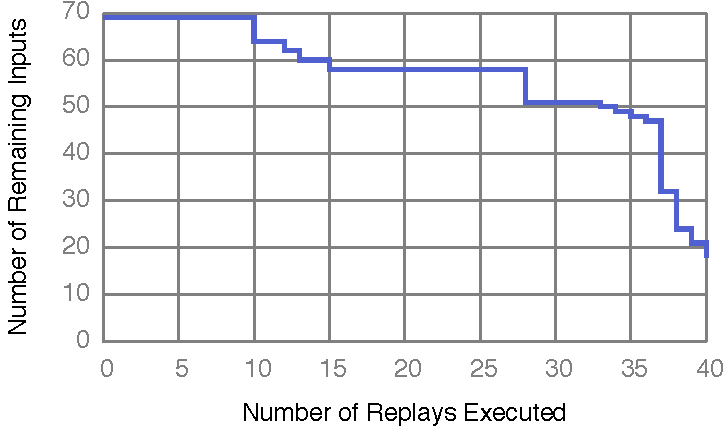
\includegraphics[width=3.25in]{../graphs/runtime/nox_loop.pdf}
    \caption[]{\label{fig:nox_discovery} Minimizing the NOX discovery loop.}
\end{figure}

Next we tested NOX on a four-node mesh, and discovered a
routing loop between three switches within
roughly 20 runs of randomly generated inputs.

Our initial input size was 68 inputs, and
\projectname~returned an 18 input MCS.\footnote{\num{We had difficulty
replaying} the final MCS. The reason seems clear: this bug depends on the
order NOX discovers links, which in turns depends on hashes computed from random memory
addresses its discovery modules LLDP selection algorithm}
Our approach to debugging was to
reconstruct from the MCS how NOX should have installed routes, then compare
how NOX actually installed routes.

The order in which NOX discovered links was crucial: at the point NOX
installed the 3-loop, it had only discovered one link towards the destination.
Therefore all other switches routed through the one known neighbor switch.
This comprised 2 of the 3 links involved in the link.

The destination host only sent one packet, which caused NOX to initially learn
its correct location. After NOX flooded the packet though, it became confused
about its location. One flooded packet arrived at
another switch that was currently not known to be attached to anything, so NOX
incorrectly concluded that the host had migrated. Other flooded packets were
dropped as a result of link failures in the network and randomly generated
network loss. The loop was then installed when the source injected another
packet.

This case took us roughly 10 hours to debug. We are confident that without the
minimized trace, it would have taken much
longer to trace through the subtle sequence of events that were necessary for
setting up the network in precisely the right conditions.

\eat{ % -----------------------------------
The next SDN control platform we examined
was NOX, the original OpenFlow controller.
NOX is also a single machine control platform, but unlike POX it has been used
fairly extensively in real networks.

Similar to POX we exercised NOX's routing module (`sprouting'), since
it draws in a large number of other components.
Routing learns link and host locations, installs all-to-all paths between
hosts on a per-flow basis, and is designed to be resilient to looped topologies.

We initially tested NOX on a two node topology, but did not find any immediate
problems. We then extended the topology to a four-node mesh, and discovered a
routing loop between two switches (involving routes for two hosts) within
roughly $20$ runs of randomly generated inputs.

Our initial input size was $150$ inputs, a minute's worth of execution.
\projectname~returned a $18$ input MCS. The most salient inputs in the
MCS were $3$ dataplane packet drops mid-way through the execution, interspersed
with $14$ traffic injections. We are in the process of pinpointing the
exact root cause with NOX developers, based on the $18$ input MCS.
} % -----------------------------------

\subsection{Floodlight discovery loop.}

\begin{figure}[t]
    %\hspace{-10pt}
    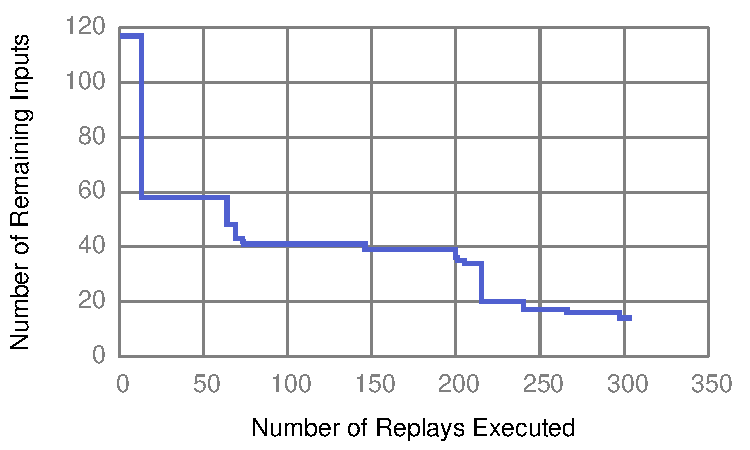
\includegraphics[width=3.25in]{../graphs/runtime/floodlight_loop.pdf}
    \caption[]{\label{fig:fl_loop} Minimizing the Floodlight loop.}
\end{figure}

We applied \projectname~to Floodlight's routing application.
In about 30 minutes, our fuzzing uncovered a
117 input sequence that caused a persistent 3-node forwarding loop.
\projectname~reduced the sequence to 13 input events in 324 replays and 8.5
hours (runtime shown in Figure~\ref{fig:fl_loop}).

We repeatedly replayed the 13 event MCS, while successively adding
instrumentation and increasing the log level each run. After about 15 replay
attempts, we found that the problem was caused by interference of end-host
traffic with ongoing link discovery packets. In our experiment, Floodlight had
not discovered an inter-switch link due to dropped LLDP packets, causing an
end-host to flap between perceived attachment points.

While this behavior cannot strictly be considered a bug in Floodlight,
the case-study nevertheless highlights the benefit of
\projectname~over traditional fuzzing techniques: by leveraging repeated replays
of a significantly reduced MCS, we were able to diagnose the root cause--a
complex interaction between the LinkDiscovery, Forwarding, and DeviceManager
modules.

\eat{ % ------------------
We subjected the current (unmodified) open
source version of Floodlight (git commit f37046a) to fuzz testing with a three
node fully meshed topology and high failure event rates. In an hour-long experiment,
the fuzzer found an event sequence with $284$ total events
that results in a 3-node forwarding loop.

Floodlight makes use of multiple kernel level
threads, and thus can exhibit non-deterministic behavior.
Thus, it is not surprising that we do not achieve full reproducibility of this
bug during replay without further instrumentation. On average, 15/50 (30\%) of
replays reproduce the bug. To proceed with MCS isolation, we replayed the
execution up to 13 replays for each subsequence chosen by delta debugging. Statistically, this enables
STS to correctly diagnose violations in >99\% of cases.\footnote{$ln( 1 -
0.99) / ln( 1 - 0.30) \approx 13$}

\projectname~was able to reduce the number of input events to $36$ input events.
Comparing output traces of successful and
unsuccessful runs, we noticed that the bug seems to correlate with specific
thread level race conditions between state updates in the \emph{LinkDiscovery} module and
the \emph{Forwarding} module. We are in the process of investigating the actual root cause.

This experiment provides a baseline for a worst case scenario of our system.
\projectname~exercised an unmodified, multithreaded controller that it does
not have deterministic control over.
The bug appears to depend on fine-grained thread-level races
conditions that are difficult to guarantee. Still, \projectname was instrumental
in pointing out a previously unknown bug, and reducing the input size.
} % ----------------------

\subsection{Known Bugs}

\subsubsection{Floodlight example failover bug}

We were able to reproduce the problem shown in Figure~\ref{fig:example} with
\projectname. We ran two Floodlight controller
instances, connected to two simulated switches, and injected 200 extraneous link
and switch failures, with the controller crash and switch connect event\footnote{We used a switch connect
event rather than a link failure event for logistical reasons, but both
can trigger the race condition} that triggered the blackhole interleaved among them.
We were able to successfully isolate the 2-event MCS.
%On ten repeated runs, the algorithm successfully pruned all extraneous
%inputs despite non-determinism in the Floodlight internal events. With full determinism and
%interposition, we expect that the algorithm should work well for less
%fabricated cases.

\subsection{Synthetic Bugs}

\url{https://docs.google.com/document/d/1l4sbpLhd7wOMhL-u6Q-zlPS5YQMLqk5ILqU7RhUxdgA/edit}.

\subsection{Overall Results.}

The overall results of our case studies are
shown in Table~\ref{tab:case_studies}.
\num{We show the initial input size and MCS input size in the last two
columns.}
For the Replay Success Rate column we
repeatedly replayed the original unpruned event trace, and measured how often we
were able to reproduce the policy violation. There was indeed non-determinism
in some cases, especially Floodlight. For the specific case of
POX in-flight blackhole, we were able to eliminate the relevant
non-determinism by employing multiplexed sockets, overriding {\tt
gettimeofday()}, and waiting on
POX's logging messages. \num{We expect that we would see similar improvements if we
applied these techniques to Floodlight.}

We measured the runtime of \projectname~for these case studies in Figures
\num{$6\;\&\;8-11$}.
While some instances ran in logarithmic time, the worst case was minimizing
the Floodlight loop,
which took more than $8.5$ hours.
%Nonetheless, we believe that even long minimization runtime
%is preferable to spending software developer's time on manual
%diagnosis.

%\subsection{Overhead}
%
%Unlike traditional record and replay techniques, \projectname (at least in
%testing mode) does not incur
%Overhead: none! Logs already there. Deterministic replay on the other
%hand has a huge overhead.

%\subsection{Mitigating Non-Determinism}
%
%Our implementation of multiplexed sockets and
%Include how many lines it took to interpose on the logging library, and how
%many lines it took to answer snapshot requests.

%\subsection{New Internal Events}
%
%How often do unexpected internal events occur in practice?
% The logging statements must also contain enough context[d] to allow for
% unambiguous fingerprinting. -> what exactly this means

\subsection{Scalability}

Mocking the network in a single process potentially prevents \projectname~from
triggering bugs that only appear at large scale. We ran
\projectname~on large FatTree networks to see where these scaling limits lie.
On a machine with 6GB of memory, we ran POX as the controller, and measured the
time to create successively larger FatTree
topologies, complete the OpenFlow handshakes for each switch,
cut $5\%$ of links, and process POX's response to the link failures. As shown in
Figure~\ref{fig:scaling}, \projectname's processing time scales roughly
linearly up to $2464$ switches (a 45-pod FatTree). At that point, the machine
started thrashing, but this limitation could easily be removed by running on a
machine with >6GB of memory.

Note that \projectname~is not designed for simulating high-throughput dataplane
traffic; we only forward what is necessary to exercise the controller
software. In proactive SDN setups, dataplane events are not
relevant for the control software, except perhaps for host discovery.

\begin{figure}[t]
    %\hspace{-10pt}
    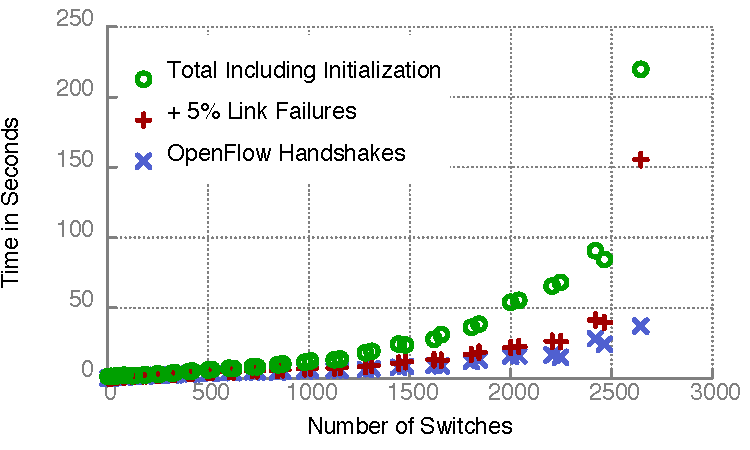
\includegraphics[width=3.25in]{../graphs/scalability/scaling.pdf}
    \caption[]{\label{fig:scaling} Simulation time for bootstrapping FatTree
    networks, cutting 5\% of links, and processing the controller's response.}
\end{figure}

\subsection{Parameters}
\label{subsec:params}

We found throughout our experimentation that \projectname~leaves open several
parameters that need to be set properly in order to effectively find and troubleshoot bugs.

\noindent{\bf Setting fuzzing parameters.} \projectname's fuzzer allows the
user to set the rates at which different event types are triggered. In our experiments with
\projectname~we found several times that we needed to set these parameters
such that we avoided bugs that were not of interest to developers.
For example, in one case we discovered that a high dataplane
packet drop rate dropped too many LLDP packets, preventing the controller from ever successfully discovering the topology.
Tweaking fuzzing parameters remains an important
part of experiment setup.

\noindent{\bf Differentiating persistent and transient violations.} In
networks there is a fundamental delay between the initial occurrence of an
event and the time when other nodes are notified of the event. This delay implies
that invariant violations such as loops or blackholes can appear
before the controller(s) have time to correct the network configuration. In
many cases such transient invariant violations are not of interest to
developers. We therefore provide a threshold parameter in \projectname~for
how long a invariant violation should persist before
\projectname~reports it as a problem. In general, setting this
threshold will depend on the parameters of the network and the invariants of
interest.

\noindent{\bf Setting \textepsilon.} Our algorithm leaves an open question as to what value
\textepsilon~should be set to. We experimentally varied \textepsilon~on the
POX in-flight blackhole and the POX list removal bugs.
We found for both cases that the number of events we timed out on while isolating the MCS became stable for values above $25$ milliseconds.
For smaller values, the number of timed out events increased rapidly. We
currently set \textepsilon~to $100$ milliseconds.

\colin{Make me work}
%\begin{table*}
%\centering
%\begin{tabular}{l|l|l|l|l|l}
%Bug Name & \textepsilon & \textepsilon & \textepsilon & \textpsilon &
%\textepsilon \\
%\hline
%POX list removal (Replay) & 59.3\% & 98.0\% & 98.3\% & 98.3\% & 98.5\% \\
%POX list removal (MCS) & 58.3\% & 69.9\% & 69.9\% & 70.6\% & 70.9\% \\
%POX in-flight blackhole (Replay) & 24.4\% & 100.0\% & 100.0\% & 100.0\% & 100.0\% \\
%POX in-flight blackhole (MCS) & 24.0\% & 75.9\% & 75.9\% & 75.9\% & 75.2\% \\
%\end{tabular}
%\caption{Percentage of Events Matched for Values of \textepsilon in ms.}
%\label{tab:epsilon}
%\end{table*}

In general, larger values of \textepsilon~are preferable to
smaller values (disregarding runtime considerations), since we can always
detect when we have waited too long (\viz~when a successor of the next input
has occurred), but we cannot detect when we have timed out
early on an internal event that is in fact going to occur shortly after.
%Analyzing event frequencies for particular bugs could provide more ideal
%\textepsilon~values.

% ------------------------------------- %
%    OLD TEXT
\eat{ % -----------------------------------

% Just realized: b/c of anonymity, the PC can't chastise us for
% running our system on our own code -- we can't tell them that it's our code!
We applied \projectname{} to three open source SDN control platforms:
Frenetic~\cite{frenetic}, POX~\cite{pox}, and Floodlight~\cite{bigswitch}, and
quickly found (or reproduced) one bug in each. The bug in Frenetic demonstrates
the utility of checking correspondence between high-level policies and
low-level configuration (without needing to specify invariants). The bugs in
POX and Floodlight demonstrate the importance of \projectname{}'s ability to
programmatically prioritize persistent correctness violations and infer their minimal
causal sets.

For all three cases, only a small code modification to the controller was necessary
to retrieve the platform's state for correspondence
checking.

\subsection{Case studies}

% Outline for bug reports:
%  - Describe each system under test
%  - Describe bugs found
%  - Lessons learned from finding bugs
Here we the discuss the three bugs we found with \projectname{}.

\noindent{\bf Frenetic.} Our first example is Frenetic~\cite{frenetic}, a control platform
providing functional-reactive language
support for programming OpenFlow networks.
Frenetic's language features aim to prevent common OpenFlow programming
errors such as race conditions and overlapping flow entries; Frenetic's
runtime system handles these low-level details on
the application's behalf. Frenetic is a modern SDN controller with a reactive
flow installation policy;
we present it here to demonstrate that \projectname{}, although focused
primarily on proactive controllers, can nonetheless be used to
troubleshoot errors in reactive control platforms.

When running learning switch, the simplest Frenetic application, we encountered
persistent correctness violations immediately. The propagation graph ($\Omega$) for Frenetic's
runtime representation of the network policy had leaves that were not present
in the physical network. Upon closer examination, we found that Frenetic's
runtime system was neglecting to remove old FLOOD routing entries from its
representation of the network policy after the hosts' route had been learned,
even though the learning switch application had
asked for these entries to be removed. Note that this case was not an overtly
malicious bug; the FLOOD entries had indeed been removed from the physical
network. The outdated controller state nevertheless went unnoticed; the bug in
Frenetic's runtime was not specific to the learning switch, and could have
resulted in failure to install flow entries at a later point in time if the
application had asked to re-install them. The key takeaway from this example
is that correspondence checking is a powerful mechanism for
verifying that the controller's representation of the network matches the true
network state correctly; without correspondence checking, troubleshooters
would need to compare the routing configurations and controller's data
structures side-by-side.

\noindent{\bf POX} Our second example is POX~\cite{pox}. POX is modeled after
Onix~\cite{onix}, a production SDN platform; as in Figure~\ref{fig:basicarch}
POX provides a physical view, a virtualized view, and a naive replication
mechanism between distributed control servers.

Because the functionality within POX is relatively young, we chose to
fabricate a bug in POX's distribution failover logic, and independently
validate that \projectname~was able to identify, prioritize, and find the
minimal causal sequence for the fabricated correctness violation.

In particular, we injected the following bug: a controller replica performs
updates to switches by (i) updating the persistent datastore storing the state
of the network (thereby notifying other replicas of the update), and (ii) pushing the
update to the switch. A control server writes a new ACL entry update to the datastore, but crashes
before completing step (ii). The switch is adopted by a new replica,
but the new control server assumes that the state in the persistent datastore
is correct. The ACL entry is therefore never installed in the switch, and a
breach of tenant isolation occurs.

We interleaved this event sequence with a normal system execution trace, and
determined whether \projectname{} could identify the correctness violation.
Throughout the system execution there were a handful of transient
correctness violations overlapping with the isolation breach. Nonetheless, our
simulator was able to identify the correct correctness violation.

\noindent{\bf Floodlight: Distributed controller failover race condition}
We were able to reproduce the problem shown in Figure~\ref{fig:example} in our
simulation environment,\footnote{The code is publicly available}
and apply \projectname~successfully.
We modified the Floodlight software to provide an interface for extracting its
physical view. We did not interpose on internal events of the controller, but instead used a
heuristic to wait for $.5$ seconds between injecting inputs to allow the
controllers to fully react. We ran two of the modified Floodlight controller
instances, connected to two simulated switches, and injected 200 extraneous link
and switch failures, with the controller crash and switch connect event\footnote{We used a switch connect
event rather than a link failure event for logistical reasons, but both
can trigger the race condition} that triggered the blackhole interleaved among them.
On ten repeated runs, the algorithm successfully pruned all extraneous
inputs despite non-determinism in the Floodlight internal events. With full determinism and
interposition, we expect that the algorithm should work well for less
fabricated cases.

\subsection{Overhead}

\colin{Reviewer OB: I would prefer to see a more in-depth analysis of why
correspondence checking is not as heavyweight as, say, conventional
model-checking. Is it the inherent symmetry in data center networks? Can we
assume that there is symmetry?}

In addition to describing bugs, we show that \projectname{} is able
to simulate and check large networks quickly.

\noindent{\bf Record and Replay Overhead.} In contrast to general record-and-replay
mechanisms, the amount of recorded state needed for
high-fidelity replay is tractable. With proactive flow installation,
updates are pushed to routing tables over a relatively long time scale; periodic
FIB snapshots along with a log of link state events, control server
downtime, and host mobility information suffice for our purposes. As a point of reference, the Cisco 7000
core switch model supports a maximum of 128K MAC entries and
128K ACL entries~\cite{cisco7000}. Assuming 36 bytes per flow entry,
(larger than the OpenFlow 13-tuple), each FIB will contain a maximum of 9216
bytes, uncompressed. A datacenter of 100,000
hosts includes roughly 8,000
switches~\cite{Al-Fares:2008:SCD:1402958.1402967}.
Therefore a snapshot of the FIBs of the entire network takes up roughly 74 MB.
The VL2 paper reports 36M network error events over one year over 8
datacenters, which implies 8.5 error events per minute per
datacenter~\cite{Greenberg:2009:VSF:1592568.1592576}.
Suppose we took a snapshot of the FIBs in the network every second.
Then we would need to store roughly 4GB, uncompressed, per minute, a relatively small growth
rate for datacenter logs. This information, in addition to a log of host
mobility events (\eg{} VM migrations) will suffice for our purposes. Note that this is a conservative overestimate.

\colin{Notes from Rean Griffith:
\begin{itemize}
\item total vms in a typical datacenter: 1000
\item migration frequency (migrations/minute): 20 per hour
\item VM spin ups/downs: 150 power ons per hour (see our OSR 2010 paper for
power off estimates)
\item Do we log VM migrations and how does that log grow (I wasn't able to
get any estimates on log-growth data)
\end{itemize}

We had an OSR 2010 paper that provided numbers scaled by the number of
VMs in an installation:
Challenges in building scalable virtualized datacenter management
(http://dl.acm.org/citation.cfm?id=1899941)
}

%To account for host mobility, assume that each server hosts 10 VMs,
%and 1\% of VMs are created, suspended, or migrated every minute. Then 10,000 host mobility events must be
%logged per minute, also a reasonable storage cost. \colin{get real numbers}

%As a point of reference, border routers' working RIB size is
%$\textasciitilde$130MB~\cite{Karpilovsky:2006:UFR:1368436.1368439}.

\noindent{\bf Correspondence Checking Runtime.} Computing the propagation
graph for correspondence checking is equivalent to enumerating
all possible paths in the network, which scales with the diameter
of the network and the number of routing entries per switch \colin{Reviewer
OC: scales how? I suspect it's at least N2}.
The propagation graph for each host can be
computed in parallel however, so the computation is bottlenecked by the serial runtime
of computing a single host's propagation graph.

We show the serial runtime of correspondence checking in
Figure~\ref{fig:hsa_runtime}. For this analysis we generated fat tree topologies
between 2 and 48 pods wide, with pre-installed PORTLAND~\cite{NiranjanMysore:2009:PSF:1592568.1592575}
routing tables in each switch. Each data point is the minimum of three
runs\colin{Reviewer OC: seems to overstate value of approach if maximum is much different} on a single Intel Xeon 2.80GHz core. Note that the number of PORTLAND routing entries per switch scales with the number
of pods in the fat-tree. We excluded the time to convert
flow tables to HSA transfer functions, since transfer functions can be maintained
offline.

\colin{Reviewer OB:  what are the characteristics of the PORTLAND routing
table? If the tables were any different, would the performance of
correspondence checking remain the same, degrade or improve? }

\colin{Reviewer OD: First the paper started generally, then it narrows its
scope to PORTLAND-style datacenters. An accurate abstract would have reflected
this narrowing of scope}

As the figure depicts, even for large networks
(27,648 hosts) the serial runtime of correspondence checking is reasonable for
interactive use. The number of serial tasks to be executed
is the number of hosts in the network squared, disregarding ECMP load balancing.
\colin{reviewer B: correspondence is not being checked. I should be clear
that this is the runtime of generating the propagation on the physical
network, which is an upper bound on the runtime of checking the virtual
network.}

\begin{figure}[t]
    %\hspace{-10pt}
    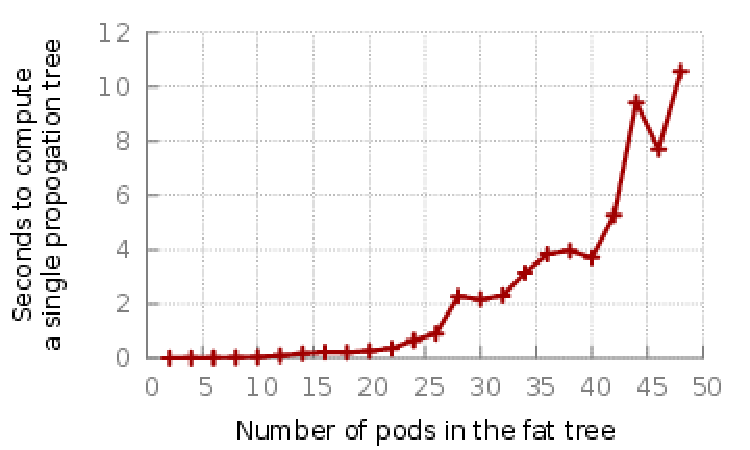
\includegraphics[width=3.25in]{../graphs/hsa_overhead_graph/graph.pdf}
    \caption[]{\label{fig:hsa_runtime} Serial runtime of correspondence
    checking on PORTLAND fat tree networks. Each datapoint consists of
    $x^3/4$ hosts and $5x^2/4$ switches (\eg{} 48 pods means 27,468 hosts
    attached to 2,880 switches)}
\end{figure}

\noindent{\bf Simulator Scalability.} Our design models the entire network
within a single process. We show in Figure~\ref{fig:scalability}
that this approach nonetheless scales to large networks. For this analysis we
generated fat tree topologies between 2 and 48 pods wide, where all switches in
the network connected to a single controller. The controller sent each switch
an OpenFlow
$FLOW\_MOD$ and subsequent $BARRIER\_REQUEST$ message, and waited for the
corresponding $BARRIER\_REPLY$. We then measured the time to between the first
$FLOW\_MOD$ sent and the last $BARRIER\_REPLY$ received. As expected, the
runtime was roughly linear with the number of switches in the network. The
figure also shows that the processing time for large networks (5 seconds per
simulator round) was well within the bounds for interactive use.

\begin{figure}[t]
    %\hspace{-10pt}
    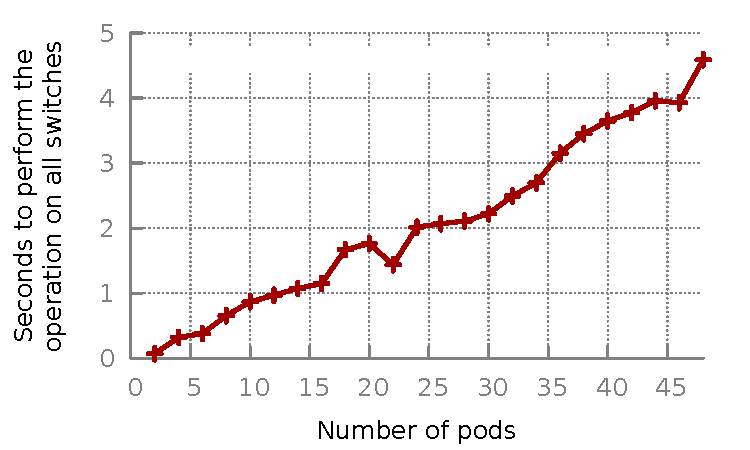
\includegraphics[width=3.25in]{../graphs/scalability_graph/scale.pdf}
    \caption[]{\label{fig:scalability} Time to send and process messages
    between controller and simulated switches. Each datapoint consists of
    $x^3/4$ hosts and $5x^2/4$ switches (\eg{} 48 pods means 27,468 hosts
    attached to 2,880 switches)}
\end{figure}

We also tested the extreme limits of the simulator's scalability, pushing up
the number of switches until something broke. We encountered what appears to be
a limitation of the Linux TCP/IP stack: TCP connection attempts began failing
beyond 26,680 sockets. Note that 26,680 switches is an order-of-magnitude larger than
the today's biggest networks.

\subsection{Replay fidelity}

On the one hand, since the SDN platform is in software, we can, in theory,
reproduce all software-induced policy violations (though not problems
resulting from flaky hardware implementing code incorrectly). However, this
requires setting up the simulator to emulate the appropriate conditions that
led to the policy violation, and that can be quite difficult. We hope to make
progress in this area along two dimensions.  First, we hope to help the
community build up a set of regression tests, so that a wide variety of
bug-triggering scenarios are available in a public repository. This would go a
long way towards providing adequate test coverage.

Second, we hope to gather error logs from real production deployments which
will help us populate this repository; this may require providing novel kinds
of anonymization, so that large datacenter operators would be willing to share
their problems (since they want their SDN code to work) without revealing the
details of their network.  This may require a infrastructural counterpart to
minimally-causal events; the smallest number of infrastructure components that
can reproduce the same bug.

Also, note that our correspondence checking algorithm can not verify
time-dependent policies such as ``No link should be congested more than 1\% of
the
time'', or ``No server should receive more than 500MB/s of external traffic''.
In future work we will extend our correspondence checking algorithm to
account for this class of policies.

\colin{reviewer B: in fact, in addition to temporal properties, the
correspondence checking algorithm cannot verify any properties involving
individual links since it only accounts for externally observable behavior!}
}    % -----------------------------------


\section{Discussion}
\label{sec:discussion}
% Just realized: b/c of anonymity, the PC can't chastise us for
% running our system on our own code -- we can't tell them that it's our code!
\Simulator{} is certainly not without limitations. We discuss several of them
here.

\noindent{\bf How big is the log? How long does this take to run?}
Assuming that it takes constant time to inject an external input, the
runtime of the algorithm is $O(n^2)$, where $n$ is the number of external inputs to
prune. If the log is too long to rerun from the beginning for
every iteration, the operator can take causally-consistent
snapshots~\cite{Chandy:1985:DSD:214451.214456} of the
live system and bootstrap the simulator from the nearest quiescent snapshot.
The length of the execution can also be `compressed' by manipulating timers in the
controllers while still maintaining happens-before dependencies.

\noindent{\bf Isn't a global log difficult to obtain?} Some failure events may appear
multiple times in the log (\eg{} replica servers detecting that a master went down),
yet we only want to replay the original event.
If it is not possible to distinguish the original
failure event from the resulting events (\eg{} in the case of a disk failure
where the original crash message is not recoverable), developers may need to
manually decipher the original event.
If the simulator is unable to reproduce the correctness violation,
the simulator may be able to `fuzz' different event
orderings in an attempt to retrigger it.

\noindent{\bf Are all simulated failures really indistinguishable
from actual failures?}
Maybe not, but since the deterministic replay environment
is built in software, the fidelity of our simulated failures
can be made arbitrarily sophisticated.\footnote{subject to scalability
limitations of fine-grained simulations}

\noindent{\bf What if there are causal dependencies between inputs events?}
Developer's need to know how the
distributed system {\it reacts} to external inputs. Understanding why external
inputs occurred is an orthogonal issue.
% POSSIBLY CUT IF NOT ENOUGH SPACE
Consider a drunk network operator who (i) trips on an ethernet cable, and
consequently (ii) spills his drink on a switch (busting the hardware). Our
system views (i) and (ii) as causally independent, and that's fine, since
the developer's goal is not to debug drunk operators.

\noindent{\bf Will this approach work on all control platforms?}
\Simulator{} requires controller-specific modifications, including
awareness of the API to specify policy changes and awareness of the format of log
messages. Correspondence checking also
assumes that it has access to views with routing table-like formats.

\noindent{\bf Will control platforms ever become stable enough that
          \simulator{} is unnecessary?}
We certainly hope so! The field is decades from that point though.

%\noindent{\bf How is this specific to SDN?}
%
%Yes!

\eat{
Second, we hope to gather error logs from real production deployments which
will help us populate this repository; this may require providing novel kinds
of anonymization, so that large datacenter operators would be willing to share
their problems (since they want their SDN code to work) without revealing the
details of their network.  This may require a infrastructural counterpart to
minimally-causal events; the smallest number of infrastructure components that
can reproduce the same bug.
}

\eat{
\colin{TODO: add note about not being able to tell difference between
endogenous and exogenous events, which might hide the true cause of a bug.
This is OK though, since we assume that the platform should always have a
correct option, but it doesn't take it. That is, the root cause of the crash
is not what we're interested in (software vs. hardware), it's how the platform
reacts to that crash that matters (should be robust, no matter what the
cause of the crash)}

\andi{Don't quite know what you mean by endogenous vs. exogenous}

\colin{Note that we also assume an out-of-band management network between
switches and controllers, and that the management network always provides 
connectivity. We could add the management network into our model if we want, I
suppose.}
}

\eat{ % The production environment logs this anyway? Add this point in
      % if we have space.
\noindent{\bf Aren't the proposed production logs going to be huge?}

In contrast to general record-and-replay
mechanisms, the amount of recorded state needed for
high-fidelity replay is tractable\andi{Check with our newly, well defined strong assumptions: 
we need full internal/external events. Is this tractable}. With proactive flow installation,
updates are pushed to routing tables over a relatively long time scale; periodic
FIB snapshots along with a log of link state events, control server
downtime, host mobility information, and policy-changes suffice for our purposes.
Assuming a maximum of 256K routing or ACL entries per switch~\cite{cisco7000}, and 
36 bytes per entry, each FIB will contain a maximum of 9216
kilobytes, uncompressed. A fat tree network of 27,648 hosts
includes 2,880
switches~\cite{Al-Fares:2008:SCD:1402958.1402967}.
Therefore a snapshot of the FIBs of the entire network would naively take up roughly
26 GB. Note however, that the data is likely to be compressible quite well, due to do its
structural and temporal properties. Assuming 8.5 error events per minute per
datacenter~\cite{Greenberg:2009:VSF:1592568.1592576}, 1,000,000
VM placement changes per day per datacenter~\cite{Soundararajan:2010:CBS:1899928.1899941},
and a small rate of human-specified policy changes, the log of the external inputs
should grow at a rate of \textasciitilde 750 entries per minute.
}

%To account for host mobility, assume that each server hosts 10 VMs,
%and 1\% of VMs are created, suspended, or migrated every minute. Then 10,000 host mobility events must be
%logged per minute, also a reasonable storage cost.

\eat{
\colin{Notes from Rean Griffith:
\begin{itemize}
\item total vms in a typical datacenter: 1000
\item migration frequency (migrations/minute): 20 per hour
\item VM spin ups/downs: 150 power ons per hour (see our OSR 2010 paper for
power off estimates)
\item Do we log VM migrations and how does that log grow (I wasn't able to
get any estimates on log-growth data)
\end{itemize}

We had an OSR 2010 paper that provided numbers scaled by the number of
VMs in an installation:
Challenges in building scalable virtualized datacenter management
(http://dl.acm.org/citation.cfm?id=1899941)
}
}

%As a point of reference, border routers' working RIB size is
%$\textasciitilde$130MB~\cite{Karpilovsky:2006:UFR:1368436.1368439}.
\eat{

TODO: Replace this analysis.
It stinks. PORTLAND is not the right way to evaluate this due to the lacking number of rules.

\noindent{\bf Correspondence Checking Runtime.} 
Computing the propagation
graph for correspondence checking is equivalent to enumerating
all possible paths in the network, which scales with the diameter
of the network and the number of routing entries per switch.
The propagation graph for each host can be
computed in parallel however, so the computation is bottlenecked by the serial runtime
of computing a single host's propagation graph.

We show the serial runtime of correspondence checking in
Figure~\ref{fig:hsa_runtime}. For this analysis we generated fat tree topologies
between 2 and 48 pods wide, with pre-installed PORTLAND~\cite{NiranjanMysore:2009:PSF:1592568.1592575}
routing tables in each switch. Each data point is the minimum of three
runs on a single Intel Xeon 2.80GHz core. Note that the number of PORTLAND routing entries per switch scales with the number
of pods in the fat-tree. We excluded the time to convert
flow tables to HSA transfer functions, since transfer functions can be maintained
offline.

As the figure depicts, even for large networks
(27,648 hosts) the serial runtime of correspondence checking is reasonable for
interactive use. The number of serial tasks to be executed
is the number of hosts in the network squared, disregarding ECMP load balancing.

\begin{figure}[t]
    %\hspace{-10pt}
    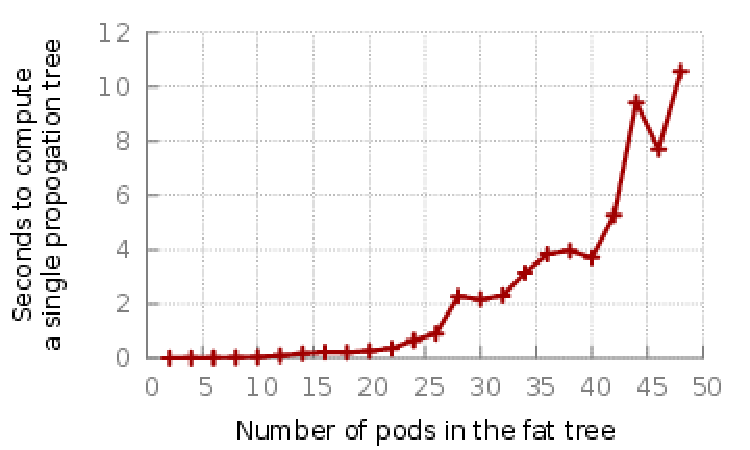
\includegraphics[width=3.25in]{../graphs/hsa_overhead_graph/graph.pdf}
    \caption[]{\label{fig:hsa_runtime} Serial runtime of correspondence
    checking on PORTLAND fat tree networks. Each datapoint consists of
    $x^3/4$ hosts and $5x^2/4$ switches (\eg{} 48 pods means 27,468 hosts
    attached to 2,880 switches)}
\end{figure}
}

\eat{ This evaluation stinks. Be gone!

\noindent{\bf Simulator Scalability.} As our approach depends on the frequently
repeating simulations, we now evaluate the setup time incurred by the simulator
system when handling large network topologies. For this experiment, shown in
Figure~\ref{fig:scalability}, we generate fat tree topologies between 2 and 48
pods wide, where all switches in the network connected to a single controller.
The controller sends each switch an OpenFlow $FLOW\_MOD$ and subsequent
$BARRIER\_REQUEST$ message, and waits for the corresponding $BARRIER\_REPLY$. We
then measure the time to between the first $FLOW\_MOD$ sent and the last
$BARRIER\_REPLY$ received. As expected, the runtime was roughly linear with the
number of switches in the network. The figure also shows that the processing
time for large networks (5 seconds per simulator round) was well within the
bounds for interactive use.

\begin{figure}[t]
    %\hspace{-10pt}
    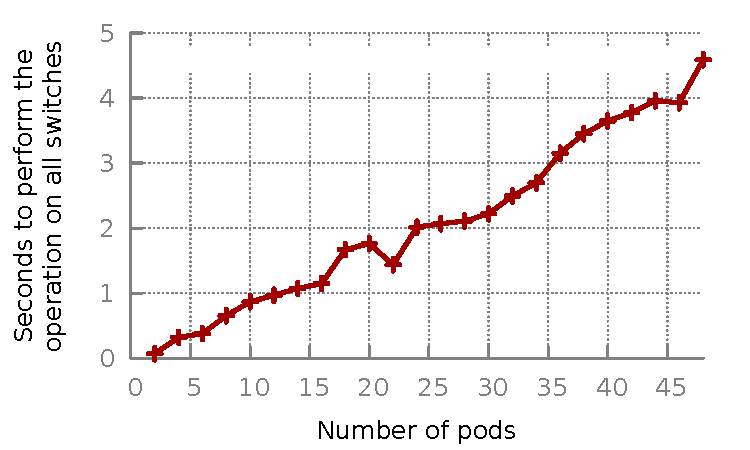
\includegraphics[width=3.25in]{../graphs/scalability_graph/scale.pdf}
    \caption[]{\label{fig:scalability} Time to send and process messages
    between controller and simulated switches. Each datapoint consists of
    $x^3/4$ hosts and $5x^2/4$ switches (\eg{} 48 pods means 27,468 hosts
    attached to 2,880 switches)}
\end{figure}

We also tested the extreme limits of the simulator's scalability, pushing up
the number of switches until something broke. We encountered what appears to be
a limitation of the Linux TCP/IP stack: TCP connection attempts began failing
beyond 26,680 sockets. Note that 26,680 switches is an order-of-magnitude larger than
the today's biggest networks.
}


\section{Related Work}
\label{sec:related_work}
%-- Program Slicing --

The delta debugging algorithm~\cite{Zeller:2002:SIF:506201.506206} seeks to solve
a problem that is exactly analogous to ours on a single machine: given input that causes a test case
to fail, what is the minimum subset of the input that still produces the failure?
We apply the same reasoning to a distributed system.

%-- Deterministic Replay (OFRewind) --

Deterministic replay techniques such as OFRewind~\cite{ofrewind}
are designed to allow developers to interactively prune
the inputs that lead up to errant behavior. We present an algorithm that
automates this process.

%-- Model checking (NICE): --

NICE~\cite{nice} combines model checking with concolic execution
to enumerate all possible code paths taken by control software (NOX)
and identify concrete inputs (\eg{} control message orderings) that cause
the network to enter invalid configurations. Unlike NICE, by analyzing
bugs {\em post-hoc} from live runs of the system our approach applies
to large software systems without suffering from state explosion.

%-- Invariant Checking? --

\eat{
Invariant checking tools such as Anteater~\cite{anteater} and HSA~\cite{hsa}
detect problems in the dataplane. We leverage invariant checking tools
to distinguish inputs that are necessary for reproducing a given invariant violation.
}

%-- Root cause analysis? --

Root cause analysis techniques~\cite{577079} seek to identify the minimum set of failed
components (\eg{} link failures) needed to explain a collection of alarms. Rather than
focusing on individual component failures, we seek to minimize inputs that affect the behavior
of the overall distributed system.

%-- Distributed Systems debuggers --

Pip~\cite{pip} is a framework for instrumenting general-purpose distributed systems
with code to record, display, and check invariants on causal paths throughout
live executions. \Simulator{} observes the causal behavior of the
distributed system in a simulated environment, enabling us to iteratively prune extraneous input events.

%-- Simulators? --
%
%Several other network simulators exist for testing SDN controllers. Mininet is a
%platform for emulating OpenFlow switches and hosts within a single
% VM~\cite{Lantz:2010:NLR:1868447.1868466}. The ns-series of network simulators
%provides a general framework for testing new protocols, topologies,
%and traffic mixes~\cite{ns3}. We found that these existing simulators did
%not provide sufficient support for the corner-cases situations which are the
%focus of our work, such as failures and VM migration.

%-- Distributed Systems --
%
%Many of our ideas originate from the literature on troubleshooting general
%distributed systems. WiDS checker introduced the notion of recording
%production executions to be later replayed and verified in a controlled simulation.
% Finally, end-to-end tracing
%frameworks such as X-Trace~\cite{Fonseca:2007:XPN:1973430.1973450} and
%Pinpoint~\cite{Chen02pinpoint:problem} provide a framework for tracing requests throughout
%a distributed system in order to infer correctness errors between layers and
%across components. Our work solves a more constrained problem; we leverage
%the structure of the SDN stack to enable a simple notion of platform
%correctness. In addition, these systems assume that invariants should hold at
%all times; we observe that in an eventually-consistent system such as SDN,
%transient policy-violations are inevitable. We built \simulator{} to help troubleshooters
%differentiate ephemeral from persistent errors.

% If we manage to run multiple applications by Monday, we should cite papers
% on consistency and cross-layer debugging:
%X-Trace~\cite{xtrace}
% Vector Clocks
% Onix
% Virtualization definitely won't happen by Monday. But, papers include
% Martin's presto '10 paper 'Virtualizaing the Network Forwarding Plane'



\section{Conclusion}
\label{sec:conclusion}
\colin{Insight to add: testing/simulation is the *main* value proposition of
SDN for Google. It is *the* main reason they have adopted it}

SDN's purpose is to make networks easier to manage. SDN
does this, however, by pushing complexity into SDN control software itself. Just
as sophisticated compilers are hard to write, but make programming easy, SDN
control software makes network management easier, but only by forcing the
developers of SDN control software to confront the challenges of asynchrony,
partial failure, and other notoriously hard problems inherent to all distributed
systems.
%Thus, people will be troubleshooting and debugging SDN control software for many
%years to come, until it becomes as stable as compilers are now.

Current techniques for troubleshooting SDN control software are primitive; they
essentially involve manual inspection of logs in the hope of identifying the
triggering inputs. Here we developed a technique for automatically
identifying a minimal sequence of inputs responsible for triggering a given
bug, without making assumptions about the language or instrumentation of the
software. We believe our technique will be especially valuable for troubleshooting
distributed controllers running complex applications, which are just now
becoming publicly available.

We focused on SDN control software, but we believe our techniques
are applicable to general distributed systems. As distributed systems
proliferate, we hope that our technique helps ameliorate the dearth of
tools in this important area.\\[0.2ex]

%We have applied this system to three open source SDN platforms.
%Of the five bugs we encountered in a five day investigation,
%our technique reduced the size of the trace to 2 inputs in the best
%case and 18 inputs in the worst case.

\eat{
SDN is widely heralded as the ``future of networking'', and its purpose is to make
it easy to manage networks. Achieving this end forces platform developers to directly
confront asynchrony, partial failure, and other problems that are inherent to all distributed
systems and notoriously difficult to get right.

In this paper we developed a technique for automatically
identifying a minimal sequence of inputs responsible for triggering a given bug.
We have applied this system to three open source SDN platforms, and
were able to find or reproduce bugs in all the platforms we investigated.
%Now we just need to provide a mechanism for the next question: would that date
%have panned out if I hadn't spilt the wine?
}

% Two ideas that have been put on the backburner:
% - distinguishing persistent violations from transient
% - using correspondence checking to localize the layer where the bug first
%   manifests

%We chose SDN as our domain becuase X,Y,Z. We envision a new paradigm where
%domain knowledge is applied to debugging in all systems.

% ------------------------------------------- %
%             OLD TEXT
\eat{
It does so by moving control plane functionality out of
network devices, and into a tightly-coupled cluster of servers that provide a simple
programmatic interface through which policies can be specified. As we have
learned in this work, the challenges of maintaining virtualized and distributed
views in a failure-prone environment are
notably different from the challenges encountered in traditional,
fully distributed control planes.

}


% TODO: Include acknowledgements section

%{\scriptsize
\bibliographystyle{abbrv} \bibliography{bib}
%}
%\input{appendix}

%\theendnotes

\end{document}
